%%%%%%%%%%%%%%%%%%%%%%%%%%%%%%%%%%%%%%%%%%%%%%%%%%%%%%%
%% Bachelor's & Master's Thesis Template             %%
%% Copyleft by Artur M. Brodzki & Piotr Woźniak      %%
%% Faculty of Electronics and Information Technology %%
%% Warsaw University of Technology, 2019-2020        %%
%%%%%%%%%%%%%%%%%%%%%%%%%%%%%%%%%%%%%%%%%%%%%%%%%%%%%%%

\documentclass[
    left=2.5cm,         % Sadly, generic margin parameter
    right=2.5cm,        % doesnt't work, as it is
    top=2.5cm,          % superseded by more specific
    bottom=3cm,         % left...bottom parameters.
    bindingoffset=6mm,  % Optional binding offset.
    nohyphenation=false % You may turn off hyphenation, if don't like.
]{eiti/eiti-thesis}

\langpol % Dla języka angielskiego mamy \langeng
\graphicspath{{img/}}             % Katalog z obrazkami.
\addbibresource{bibliografia.bib} % Plik .bib z bibliografią

\begin{document}

%--------------------------------------
% Strona tytułowa
%--------------------------------------
\MasterThesis % Dla pracy inżynierskiej mamy \EngineerThesis
\instytut{Systemów Elektronicznych}
\kierunek{Elektronika}
\specjalnosc{Mikrosystemy i Systemy Elektroniczne}
\title{
    Implementacja sztucznych sieci neuronowych w systemach\\
    SoC i MPSoC z wykorzystaniem akceleratorów, realizowanych\\w technice HLS
}
\engtitle{ % Tytuł po angielsku do angielskiego streszczenia
    Artificial Neural Networks implementation in SoC and MPSoC systems using 
    accelerators synthesized by HLS method
}
\author{Krzysztof Wasilewski}
\album{265956}
\promotor{dr inż. Wojciech Zabołotny}
\date{\the\year}
\maketitle

%--------------------------------------
% Streszczenie po polsku
%--------------------------------------
\cleardoublepage % Zaczynamy od nieparzystej strony
% \setcounter{page}{1} % W szablonie nie było tej linii i strona tytułowa była numerowana

\streszczenie
Sztuczne Sieci Neuronowe są w dzisiejszych czasach wykorzystywane w wielu 
zastosowaniach. Duża złożoność algorytmów Sztucznej Inteligencji wymaga 
dużej mocy obliczeniowej oraz odpowiednich metod optymalizacji 
i właściwego wyboru sprzętu. W przypadku obliczeń, które można 
zrównoleglić, rozsądnym wyborem są układy FPGA (ang. \emph{Field Programmable Gate 
Array}). 

Głównym celem pracy było zaprojektowanie i implementacja sztucznej sieci
neuronowej przy wykorzystaniu systemu SoC (ang. \emph{System on Chip}) z układem 
FPGA i techniki HLS (ang. \emph{High Level Synthesis}). Użycie techniki HLS
pozwala na projektowanie przy wykorzystaniu języka C, C++ lub System 
C i umożliwia korzystanie z wielu bibliotek zaimplementowanych w języku 
C i C++, co znacznie przyspiesza pracę nad projektem.

Założeniem pracy było stworzenie akceleratora, umożliwiającego osiągnięcie
wzrostu wydajności algorytmu detekcji obiektów znajdujących się na 
obrazie w czasie rzeczywistym. W~ostatnich latach można zaobserwować 
wielki postęp w dziedzinie komputerowego rozpoznawania obrazów 
(ang. \emph{Computer Vision}), jednak większość dostępnych implementacji jest 
przeznaczona do uruchomienia na komputerze PC.

\slowakluczowe Sztuczne Sieci Neuronowe, HLS, komputerowe rozpoznawanie 
obrazów, FPGA

%--------------------------------------
% Streszczenie po angielsku
%--------------------------------------
\cleardoublepage  % Zaczynamy od nieparzystej strony

\abstract
Nowadays, Artificial Neural Networks (ANN) are used in many applications. 
High complexity of Artificial Intelligence algorithms requires high 
computing power, appropriate optimization methods and efficient hardware. 
In the case of computation that is easy to parallelize it is reasonable 
to use FPGA systems.

The main aim of the thesis was to design and implement an Artificial 
Neural Network algorithm using SoC (System on Chip) with FPGA system 
and HLS (High-Level Synthesis) method. HLS method allows to design a 
project using C, C++ or System C language and use lots of C libraries, 
which makes working on the project faster.


Assumption was made that the created accelerator will allow to achieve 
efficiency improvement in the real-time object detection algorithm. 
Recently, it is seen that huge improvement was made in the field of 
Computer Vision, but most of the available implementations are made to 
run on PC.

\keywords Artificial Neural Networks, HLS, Computer Vision, FPGA

%--------------------------------------
% Oświadczenie o autorstwie
%--------------------------------------
\cleardoublepage  % Zaczynamy od nieparzystej strony
\pagestyle{plain}
\makeauthorship
% \setcounter{page}{2}
%--------------------------------------
% Spis treści
%--------------------------------------
\cleardoublepage % Zaczynamy od nieparzystej strony
\tableofcontents

%--------------------------------------
% Rozdziały
%--------------------------------------
\cleardoublepage % Zaczynamy od nieparzystej strony
\pagestyle{headings}

\newpage % Rozdziały zaczynamy od nowej strony.
\cleardoublepage % Zaczynamy od nieparzystej strony
\pagestyle{headings}
\section{Wstęp}

\subsection{Wprowadzenie}

W ostatnich latach można zaobserwować gwałtowny rozwój w dziedzinie 
Uczenia Maszynowego (ang. \emph{Machine Learning}) i Sztucznej Inteligencji 
(ang. \emph{Artificial Intelligence}). Coraz więcej urządzeń i systemów projektowanych jest w sposób zapewniający działanie autonomicznie, bez potrzeby ingerencji człowieka. 
Jednym z algorytmów, który powstał już dość dawno, są Sztuczne Sieci Neuronowe (ang. \emph{Artificial Neural Networks}). Temat Sieci Neuronowych ma długą historię rozwoju, sięgającą początku lat 40. XX wieku, jednak w ostatnich latach można zaobserwować znaczny postęp w tej dziedzinie \cite{Kriesel2007NeuralNetworks}. Rozwój technologii umożliwił zastosowanie algorytmów AI w wielu aplikacjach. Działalność naukowa w kierunku Sztucznych Sieci Neuronowych spowodowała powstanie nowych modeli i architektur.

Większość algorytmów wykorzystujących Sztuczną Inteligencję wymaga dużej mocy 
obliczeniowej i wyboru odpowiedniego sprzętu. Często powtarzaną operacją matematyczną 
w przypadku algorytmu Sztucznej Sieci Neuronowej jest mnożenie macierzy.
Działanie to można w łatwy sposób zrównoleglić, implementując sieć w układzie 
FPGA i tym samym zwiększyć efektywność algorytmu.

Praca nad implementacją algorytmów Sztucznej Inteligencji w większości 
przypadków zaczyna się od stworzenia i uruchomienia modelu. Do tego zadania 
często wykorzystywane są wysokopoziomowe biblioteki takie jak \emph{keras} lub \emph{Theano}, które w znacznym stopniu przyspieszają proces tworzenia oprogramowania oraz ułatwiają wprowadzanie zmian w modelu sieci. Rozwój i dopracowywanie 
algorytmu Sztucznej Inteligencji wymaga wielu iteracji uruchamiania kodu 
z różnymi parametrami i właściwościami sieci. Aby w~pełni wykorzystać potencjał Sztucznych Sieci Neuronowych, należy dobrać odpowiednio metody projektowania i testowania modeli.

\subsection{Wstęp teoretyczny}

Sieć neuronowa jest algorytmem przetwarzającym dane, inspirowanym działaniem mózgu. ANN składa się z wielu elementów przetwarzających informacje -- neuronów. Model przetwarzania informacji jest inspirowany ludzkim mózgiem jednak w stosunku do komórki nerwowej, neuron w Sztucznej Sieci Neuronowej jest bardzo uproszczony
\cite{tadeusiewicz1993sieci}. Pomimo to ANN umożliwiają rozwiązywanie złożonych
problemów w wielu dziedzinach z~dużą dokładnością.

Pomiędzy neuronami prowadzone są połączenia, z których każde ma swoją wagę, która 
zmienia wartość w trakcie uczenia sieci. Warstwę sieci, w której wszystkie wyjścia każdego z neuronów są podłączone do wszystkich neuronów w warstwie następnej, nazywa się warstwą w pełni połączoną (ang. FC — \emph{Fully Connected}).
Sieć posiadająca wszystkie warstwy w pełni połączone jest zwana siecią w pełni połączoną. 

W znacznej większości sieci neuronowe budowane są w ten sposób, że dane są propagowane w kierunku od warstwy wejściowej do wyjściowej. Takie sieci nazywamy sieciami jednokierunkowymi (ang. \emph{feedforward}). Przykładową sieć neuronową w pełni połączoną typu \emph{feedforward} przedstawiono na Rys. \ref{ann-img}.
\bigskip

\begin{figure}[h]
  \centering
  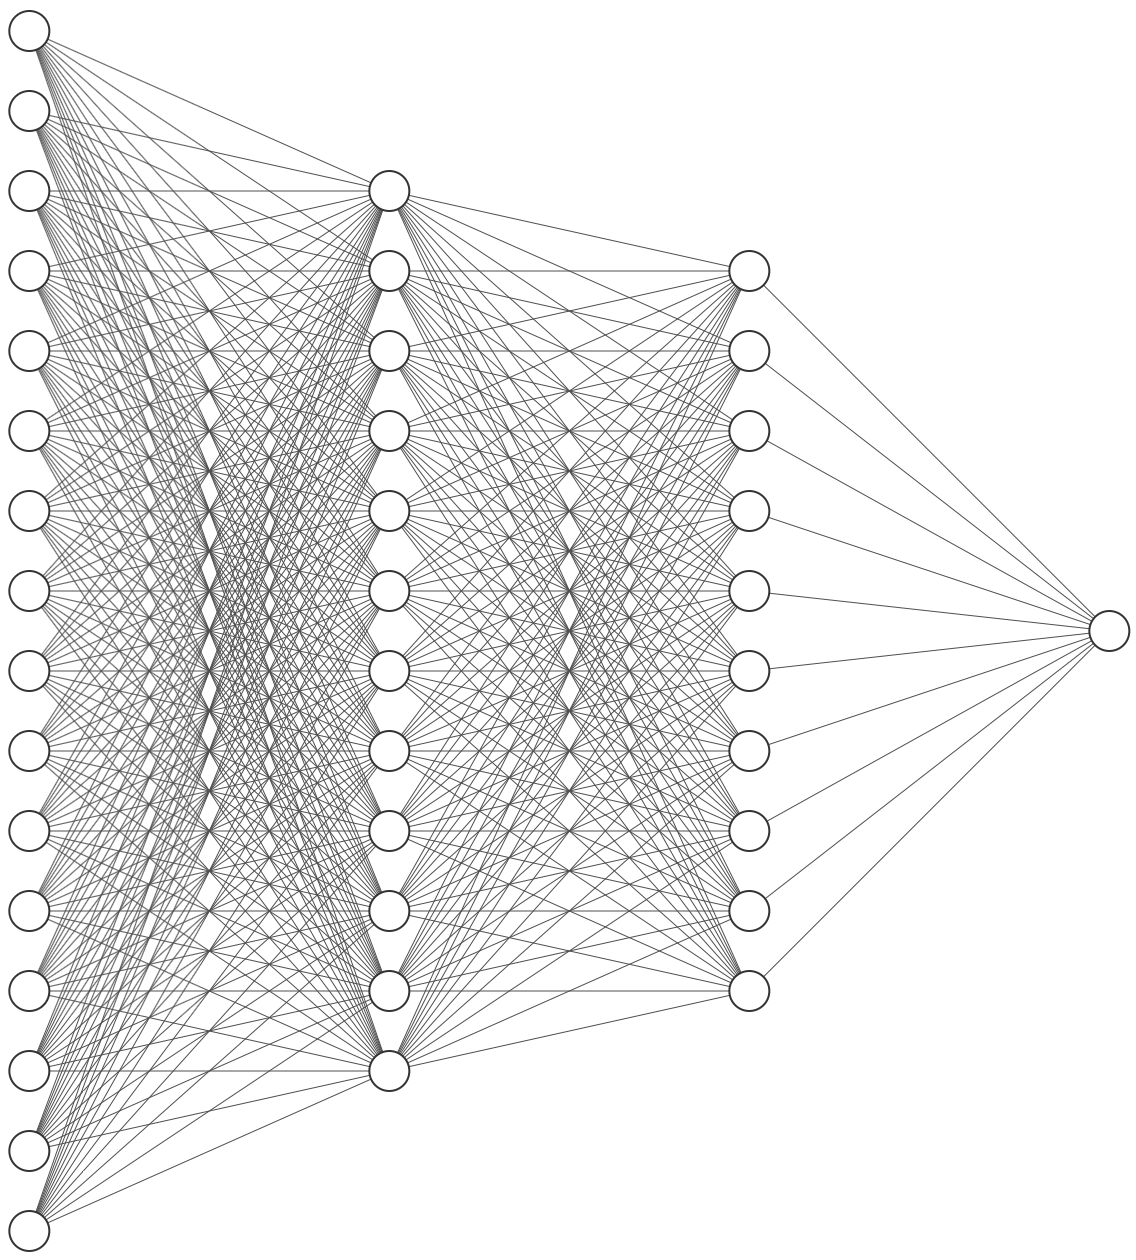
\includegraphics[width=0.8\textwidth]{img/ann.png}
  \caption{Schemat w pełni połączonej jednokierunkowej Sieci Neuronowej (wygenerowany na stronie: \url{http://alexlenail.me/NN-SVG/})}
  \label{ann-img}
\end{figure}


\subsubsection{Model neuronu}
Sztuczne Sieci Neuronowe to algorytm inspirowany działaniem ludzkiego mózgu 
i~znajdujących się w nim neuronów. Model matematyczny (Rys. \ref{neuron}) pojedynczego neuronu składa się z następujących elementów \cite{Omondi2006FPGAIO}:
\begin{itemize}
  \item wektora wejściowego: 
  $$x = (x_1, x_2,...,x_j)^T$$
  \item wektora wag przypisanych do każdego z wejść
  $$w = (w_{k1}, w_{k2},...,w_{kj})^T$$
  \item wyrazów wolnych (bias) $b$
  \item funkcji aktywacji $\phi(u)$ 
  \item wyjścia neuronu $y$. 
\end{itemize}
Wyrazy wolne (bias) umożliwiają kontrolowanie progu aktywacji neuronu, niezależnie od wartości wejściowych. W praktyce oznacza to przesuwanie wykresu funkcji aktywacji w~zależności od znaku w prawą lub w lewą stronę. Wyjście neuronu można policzyć, stosując następujące wzory:
$$u_k = \sum_{j=1}^{N}{w_{kj}x_j} $$ 
$$y_k = \phi(u_k + b_k) $$ 

Najprostsza Sieć Neuronowa składająca się z jednego neuronu, nazywana jest \emph{Perceptronem}. Algorytm ten można wykorzystać do zadań klasyfikacji binarnej.

\begin{figure}[h]
  \centering
  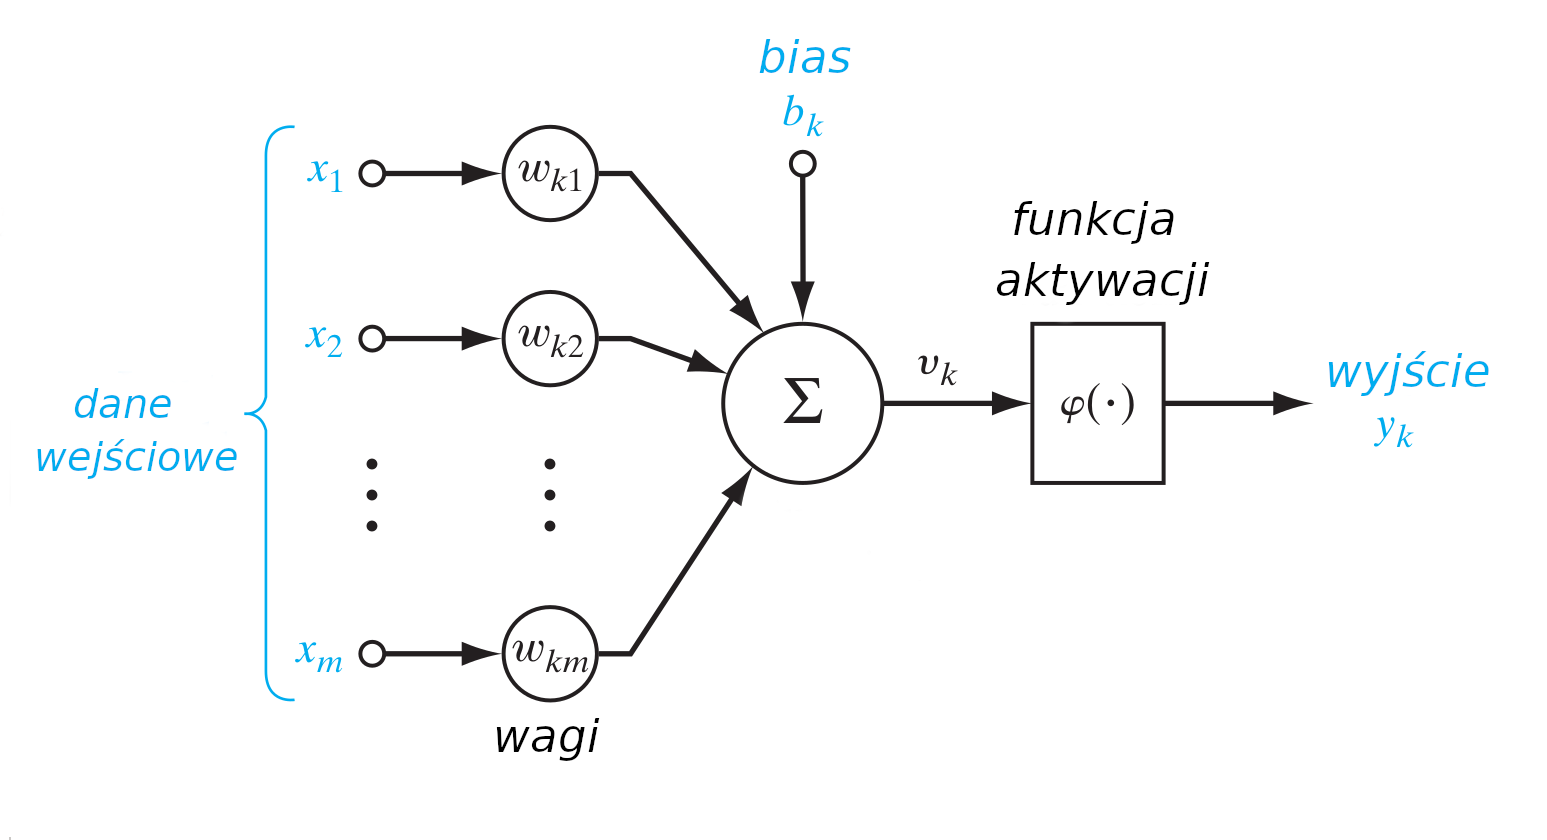
\includegraphics[width=\textwidth]{img/neuron.png}
  \caption{Model neuronu \cite{haykin2009neural}}
  \label{neuron}
\end{figure}


\subsubsection{Funkcja aktywacji}
Na działanie algorytmu znaczny wpływ może mieć dobór odpowiedniej 
funkcji aktywacji. Wśród najczęściej stosowanych funkcji aktywacji
wyróżnia się następujące funkcje:
\begin{itemize}
    \item funkcja ReLu (ang. \emph{Rectified Linear Units}): 
    
    $$\phi(x) = max(0, x)$$
    
    \begin{figure}[!h]
      \centering
      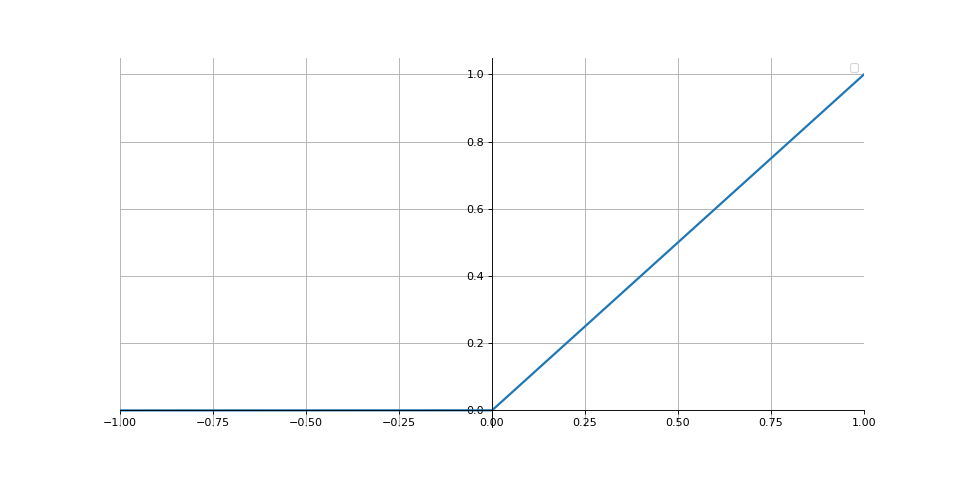
\includegraphics[width=\textwidth]{img/relu.png}
      \caption{Wykres funkcji ReLU}
      \label{relu}
    \end{figure}

    \item funkcja sigmoid: 
    
    $$\phi(x) = \frac{a}{a + e^{-bx}}$$
    
    \begin{figure}[!h]
      \centering
      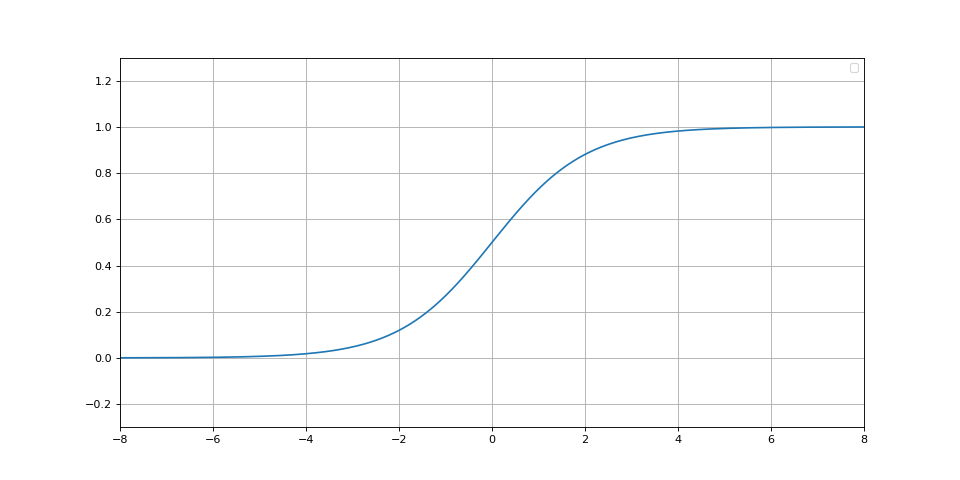
\includegraphics[width=\textwidth]{img/sigmoid.png}
      \caption{Wykres funkcji sigmoid}
      \label{sigmoid}
    \end{figure}
    
    \item funkcja softmax (liczona dla każdego neuronu warstwy wyjściowej, j = 1,...,N): 
    $$\phi(x_j) = \frac{e^{x_j}}{\sum_{k=1}^{N}{e^{x_k}}}$$
\end{itemize}

W warstwach ukrytych często używaną funkcją aktywacji jest funkcja ReLU oraz sigmoid. Funkcję sigmoid stosuje się również w warstwach wyjściowych przy zadaniach klasyfikacji binarnej. Funkcja softmax jest używana w problemach klasyfikacji wieloklasowej (np. rozpoznawanie cyfr). Stosując funkcję softmax w warstwie wyjściowej, można traktować wektor wartości wyjść sieci jako rozkład prawdopodobieństwa wyboru danego rozwiązania.

\subsubsection{Perceptron wielowarstwowy}
Jednym z pierwszych modeli Sztucznych Sieci Neuronowych był Perceptron
Wielowarstwowy (ang. MLP — \emph{Multi-Layer Perceptron}), składający 
się z warstwy neuronów wejściowej, ukrytych i wyjściowej (Rys.\ref{mlp}).
Wyjście neuronów w danej warstwie staje się wejściem neuronów warstwy następnej.

Sieć Neuronowa typu MLP najczęściej posiada warstwy w pełni połączone
(ang. FC -- \emph{Fully Connected}) lub inaczej Gęste (ang. \emph{Dense}). W warstwie FC każde z wyjść jest podłączone do wszystkich wejść neuronów w warstwie następnej.

\begin{figure}[h]
  \centering
  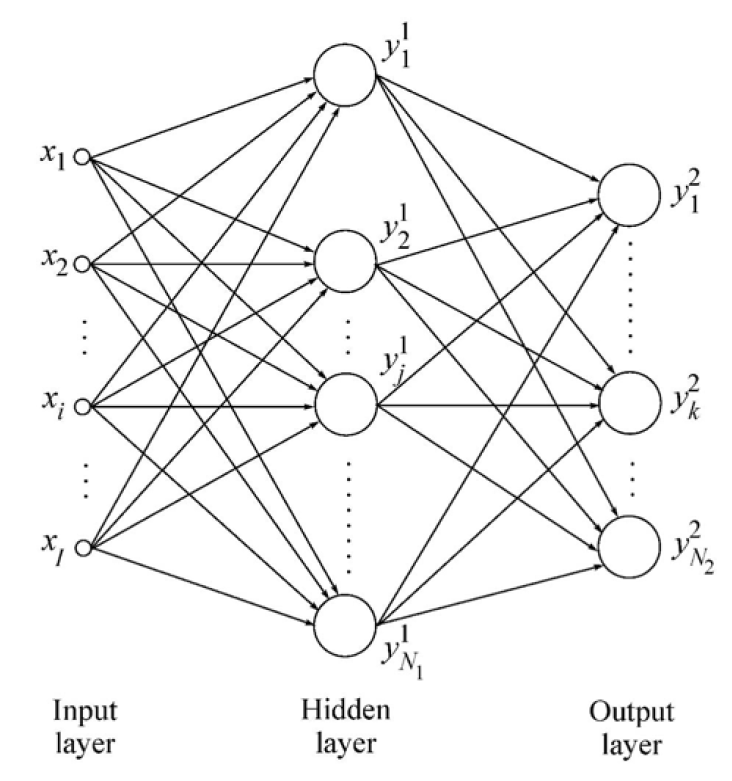
\includegraphics[width=\textwidth]{img/mlp.png}
  \caption{Model Perceptronu Wielowarstwowego}
  \label{mlp}
\end{figure}


\subsubsection{Sieci Głębokie}

Rozwój algorytmów AI doprowadził do powstania Głębokich Sieci Neuronowych (ang. 
\emph{DNN — Deep Neural Networks}), czyli takich, które posiadają wiele 
warstw ukrytych \cite{Goodfellow-et-al-2016}. Algorytm Uczenia Głębokiego (ang. 
\emph{Deep Learning}) umożliwia rozwiązywanie skomplikowanych problemów takich 
jak rozpoznawanie i klasyfikację obiektów na obrazie (Rys.\ref{dnn}). Seria warstw ukrytych (ang. \emph{hidden layers}) umożliwia ekstrakcję cech obiektów. 
Kolejne warstwy umożliwiają wykrywanie krawędzi, potem konturów, a na końcu 
całych kształtów i obiektów.

\begin{figure}[!h]
  \centering
  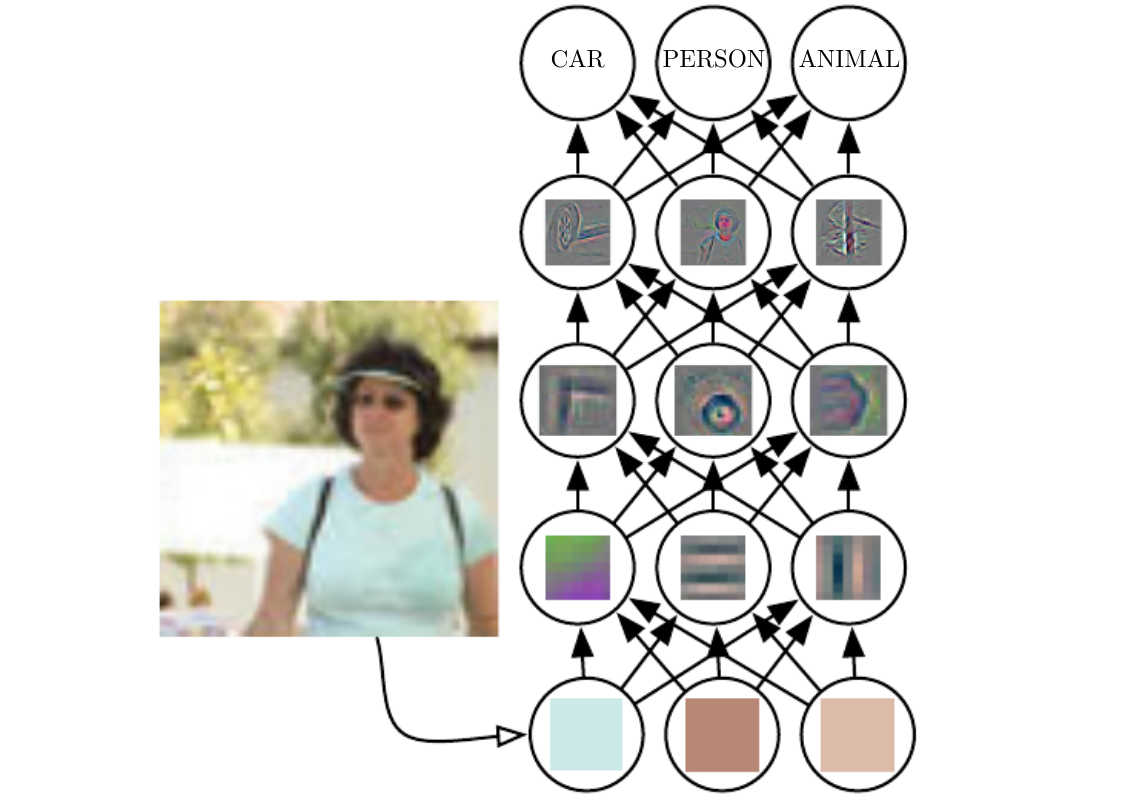
\includegraphics[width=\textwidth]{img/dnn-object-recog.png}
  \caption{Model Głębokiego Uczenia sieci \cite{Goodfellow-et-al-2016}}
  \label{dnn}
\end{figure}


\subsubsection{Proces uczenia sieci}

Uczenie Sztucznej Sieci Neuronowej można podzielić na nadzorowane (ang. \emph{supervised learning}) i nienadzorowane (ang. \emph{unsupervised learning}) oraz wersję pośrednią -- uczenie częściowo nadzorowane (ang. \emph{semi-supervised learning}). W praktyce najczęściej wykorzystywanym rodzajem uczenia jest \emph{supervised learning}, jednak uczenie nienadzorowane, które zakłada tworzenie modelu sieci bez ingerencji człowieka, jest ciekawym tematem badań i rozwoju algorytmów Sztucznych Sieci Neuronowych \cite{nielsen2015neural}.
Proces uczenia nadzorowanego sieci polega na zwiększaniu dokładności ANN w rozwiązywaniu danego problemu. Odbywa się to poprzez iteracyjne korygowanie wartości wag i wyrazów wolnych (bias) tak, aby zminimalizować błąd pomiędzy rozwiązaniem wzorcowym i otrzymanym. Jeden z algorytmów zmiany wag podczas uczenia jest reguła delty (ang. \emph{delta rule}):


$$\Delta w_{kj} = \eta e_k(n)x_j(n) $$
$$ e_k(n) = d_k(n) - y_k(n) $$

W powyższym wzorze $d_k(n)$ jest zakładanym rozwiązaniem, a $y_k(n)$ rozwiązaniem otrzymanym.
Wartość $\eta$ oznacza współczynnik szybkości uczenia (ang. \emph{learning rate}). Gdy jest wystarczająco mały, algorytm uczenia osiąga rozwiązanie optymalne, jednak większy współczynnik $\eta$ może przyspieszyć ten proces. Wpływ na szybkość uczenia ma również wielkość miniserii (ang. \emph{mini-batch}) uczących. Jest to liczba elementów zbioru uczącego, podawanych na wejście algorytmu, przed zaktualizowaniem wartości wag sieci. Z powodu ograniczonych rozmiarów zboru uczącego, jest on wykorzystywany wielokrotnie. Jedno przejście przez wszystkie próbki ze zbioru uczącego nazywane jest epoką (ang. \emph{epoch}) \cite{tadeusiewicz2015leksykon}.

\subsubsection{Wsteczna propagacja błędu}
Architekturę sieci MLP często stosuje się wraz z algorytmem wstecznej 
propagacji błędu (ang. \emph{Backpropagation}), która umożliwia proces uczenia sieci. Poprzez obliczenie błędu w neuronach warstwy wyjściowej i propagacji wstecz błędu przez całą sieć, algorytm pozwala dostosować wartość wagi każdego z połączeń w taki sposób, aby zminimalizować wartość funkcji kosztu. Sieć jest uczona do momentu, gdy błąd stanie się akceptowalnie mały. 

\subsubsection{Hiperparametry}
W procesie uczenia Sztucznej Sieci Neuronowej bardzo istotne jest odpowiednie ustawienie parametrów sieci, zwanych hiperparametrami (ang. \emph{hyperparameters}). Są to parametry sieci, ustawiane przez użytkownika w celu otrzymania modelu, dającego najlepsze rozwiązania. Na wynik uczenia wpływ mają m.in. następujące Hiperparametry:
\begin{itemize}
  \item liczba i rodzaj warstw sieci
  \item liczba neuronów w każdej z warstw
  \item współczynnik szybkości uczenia $\eta$
  \item wielkość miniserii
  \item liczba epok.
\end{itemize}

\subsubsection{Przeuczenie sieci}

Przy używaniu Sztucznych Sieci Neuronowych w zadaniach klasyfikacji często spotykanym problemem jest przeuczenie sieci (ang. \emph{overfitting}). Przeuczona sieć jest zbyt mocno dopasowana do danych uczących i przy walidacji poprawność klasyfikacji jest znacznie mniejsza. Jednym ze sposobów na polepszenie zdolności do generalizacji trenowanego modelu sieci jest zastosowanie \emph{Dropoutu}, czyli losowego usuwania pewnej ustalonej liczby neuronów. Technika ta, pomimo swojej prostoty, daje bardzo dobre wyniki w~przeciwdziałaniu przeuczeniu sieci.  

\subsubsection{Splotowe Sieci Neuronowe}

Splotowe Sieci Neuronowe (ang. \emph{CNN -- Convolutional Neural Networks}) są typem sieci głębokich, które znakomicie nadają się do rozpoznawania kształtów i z powodzeniem stosowane w wielu zagadnieniach klasyfikacji obrazów. Charakteryzują się dużą odpornością na rotację, skalowanie, zniekształcanie i inne zakłócenia \cite{haykin2009neural}. Sieci te są uczone w trybie nadzorowanym. 

Za ekstrakcję cech obiektów w dwuwymiarowym obrazie odpowiedzialna jest warstwa splotowa sieci. Wejście \textbf{\emph{M}} tej warstwy jest przekształcane przy użyciu odpowiedniego filtru \textbf{\emph{K}}. Operację splotu w sieciach CNN można opisać wzorem:
$$
S(i,j) = (M*K)(i,j) =\sum_{k}{\sum_{j}{M(i - k, j - l)K(k, l)}}
$$

Wynik \textbf{\emph{S(i,j)}} nazywany jest mapą atrybutów (ang. \emph{feature map}). Warstwa splotowa umożliwia zmniejszenie rozmiaru przetwarzanych danych podczas uczenia sieci oraz zwiększa jej zdolność do generalizacji. Operację splotu przedstawiono na Rys. \ref{conv}. Zaprezentowany przypadek to splot macierzy 6x6 przy użyciu filtru o rozmiarze 3x3. 


\begin{figure}[!h]
  \centering
  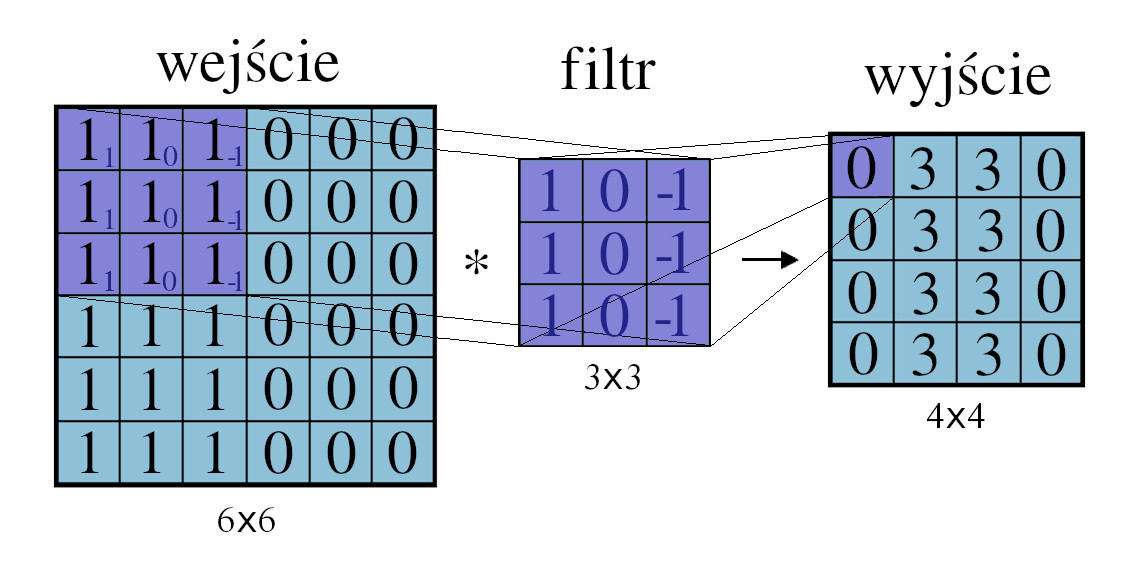
\includegraphics[width=\textwidth]{img/conv.jpg}
  \caption{Splot macierzy 6x6 przy użyciu filtru o rozmiarze 3x3}
  \label{conv}
\end{figure}


Razem z warstwą splotową często stosowana jest warstwa grupowania (ang. \emph{pooling}), występującą najczęściej w jednym z dwóch wariantów (ang. \emph{max-pooling}) lub (ang. \emph{average pooling}). W przypadku przetwarzania obrazu metoda (ang. \emph{max-pooling}) polega na zmniejszeniu jego rozmiaru, poprzez wybranie wartości maksymalnej lub średniej, stosując okno o wybranym rozmiarze. Najczęściej wybieranym krokiem (ang. \emph{stride}) przesuwania okna jest wartość, równa jego rozmiarowi. Na Rys. \ref{pooling} przedstawiono przykład \emph{max-poolingu} o rozmiarze 2x2 ze skokiem równym rozmiarowi okna.

\begin{figure}[!h]
  \centering
  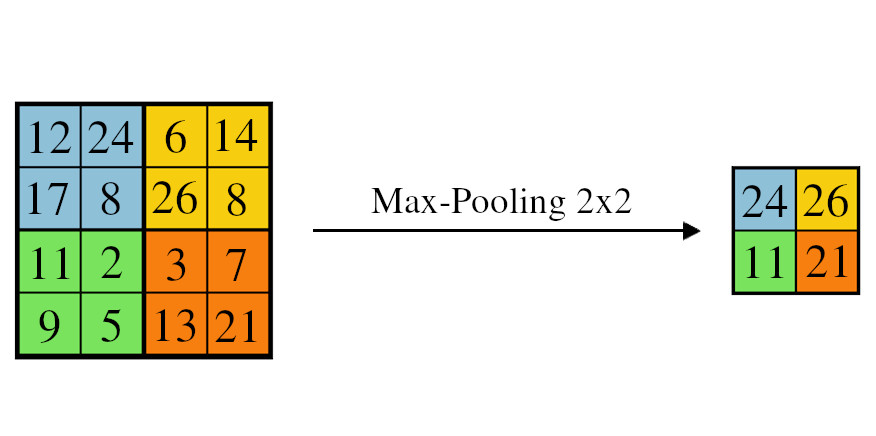
\includegraphics[width=\textwidth]{img/pooling.jpg}
  \caption{Max-pooling o rozmiarze 2x2}
  \label{pooling}
\end{figure}

\subsection{Zastosowania Sztucznych Sieci Neuronowych}

W dzisiejszych czasach Sztuczne Sieci Neuronowe są wykorzystywane w wielu zastosowaniach. Dziedziny, w których stosuje się algorytmy ANN to m.in.:
\begin{itemize}
  \item medycyna -- wspomaganie wystawiania diagnozy
  \item przemysł -- automatyczna kontrola jakości produktów
  \item zastosowania militarne -- wspomaganie radarów i termowizji
  \item ekonomia -- przewidywanie notowań giełdowych
  \item robotyka -- autonomiczne samochody (Rys. \ref{self-driving-car})
  \item rozpoznawanie i synteza mowy -- sterowanie różnymi systemami (smartfon, komputer, urządzenia IoT) przy użyciu asystenta głosowego
\end{itemize}

\begin{figure}[!h]
  \centering
  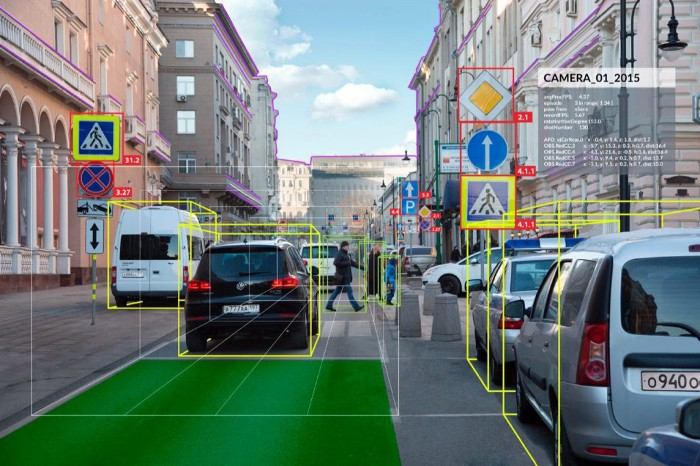
\includegraphics[width=\textwidth]{img/self-driving-car.jpg}
  \caption{Rozpoznawanie obiektów na obrazie z kamery samochodu autonomicznego \cite{self-drive-obraz}}
  \label{self-driving-car}
\end{figure}

                      % Wygodnie jest trzymać każdy rozdział w osobnym pliku.
\newpage % Rozdziały zaczynamy od nowej strony.
\cleardoublepage % Zaczynamy od nieparzystej strony
\pagestyle{headings}

\section{Cel i zakres pracy}
Celem pracy było zaprojektowanie i implementacja sztucznej sieci neuronowej 
przy wykorzystaniu systemu SoC (ang. System on Chip) i techniki HLS. 
Użycie metody HLS umożliwia projektowanie przy wykorzystaniu języka 
C, C++ lub System C oraz co zazwyczaj skraca czas wykonania projektu.  
Dodatkowo HLS umożliwia korzystanie z wielu bibliotek, zawierających funkcje, wykorzystywane w implementacji 
Sztucznych Sieci Neuronowych. Oczekiwanym wynikiem pracy było stworzenie akceleratora, umożliwiającego osiągnięcie 
wzrostu wydajności w stosunku do rozwiązań software’owych uruchamianych na komputerze PC.

\subsection{Motywacja}
Sztuczne Sieci Neuronowe są związane z dużą ilością obliczeń, które mogą 
być wykonywane równolegle. Pozwala to osiągnąć krótszy czas wykonania 
programu, co ma duże znaczenie dla zastosowań w systemach działających 
w czasie rzeczywistym np. w branży \emph{Automotive}. Aby osiągnąć przyspieszenie 
obliczeń, stosuje się różne metody. Jednym z najpopularniejszych obecnie sposobów 
na zwiększenie wydajności algorytmów AI jest wykorzystanie kart graficznych GPU 
(ang. \emph{Graphics Processing Unit}). Metodą najbardziej przyspieszającą obliczenia,
lecz wymagającą najdłuższego czasu projektowania i najbardziej kosztowną,
jest zastosowanie specjalizowanych układów ASIC (ang. \emph{Application-Specific 
Integrated Circuit}). Opcją pośrednią pomiędzy powyższymi dwoma rozwiązaniami
jest zastosowanie układów FPGA. To podejście umożliwia osiągnięcie znacznego
przyspieszenia wykonywania obliczeń i nie powoduje wielkiego wzrostu kosztów. 
Dodatkowo zastosowanie metody HLS ułatwia i minimalizuje czas tworzenia sprzętowej 
implementacji modelu ANN oraz wprowadzanie zmian w projekcie. Implementacja danego algorytmu może być optymalizowana pod kątem zużycia zasobów oraz wprowadzanych opóźnień przy użyciu dyrektyw kompilatora Vivado HLS. Dzięki temu programista posiadający minimalną wiedzę o sprzęcie jest w stanie utworzyć implementację dającą zadowalające rezultaty.

\subsection{Układy GPU i FPGA w zastosowaniach \emph{Machine Learning}}
W większości przypadków Sztuczne Sieci Neuronowe są projektowane, uczone i uruchamiane na procesorze z akceleratorem obliczeń 
w postaci GPU. Jednak wydajne układy graficzne nie zawsze są dostępne w systemach wbudowanych oraz wprowadzają dodatkowe koszty systemu i duże zużycie mocy.

Alternatywnym sposobem na przyspieszenie obliczeń związanych z implementacją algorytmów ANN jest zastosowanie układów FPGA. Dodatkowym atutem po stronie układów FPGA jest mniejsze zużycie mocy. Dzięki odpowiednim metodom optymalizacji, przy wykorzystaniu układów FPGA można osiągnąć znacznie mniejsze zużycie zasobów i przyspieszenie obliczeń.

Przewagą zastosowania układów GPU jest łatwość implementacji skomplikowanych obliczeń dzięki zastosowaniu architektury \emph
{CUDA} (ang. \emph{Compute Unified Device Architecture}), opracowanej przez firmę \emph{Nvidia}. Dzięki CUDA, zrównoleglenie obliczeń jest możliwe przy użyciu języków programowania takich jak C, C++, Fortran, Python i MATLAB \cite{cuda} i nie wymaga tyle wiedzy o sprzęcie co użycie metody HLS. Pomimo to technika HLS jest cały czas rozwijana. Powstają narzędzia dedykowane do zastosowań akceleracji obliczeń w Sztucznych Sieciach Neuronowych. W trakcie pisania tej pracy pojawiło się nowe narzędzie producenta \emph{Xilinx} -- \emph{Vitis AI}, zapewniające wsparcie w tworzeniu rozwiązań ML z użyciem układów FPGA. \emph{Vitis AI} jest zbiorem bibliotek i API (ang. \emph{Application Programming Interface}) stworzonym do zastosowań wydajnego uruchamiania algorytmów AI \cite{vitis-ai}. To pokazuje, że synteza wysokiego poziomu w układach FPGA charakteryzuje się pozytywną tendencją rozwoju.

\begin{figure}[h]
    \centering
    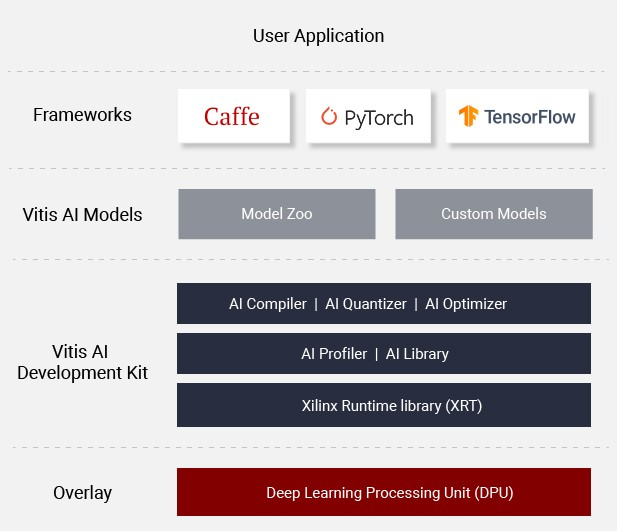
\includegraphics[width=\textwidth]{img/vitis-AI.jpg}
    \caption{Struktura narzędzia Vitis-AI \cite{vitis-AI-obraz}}
    \label{vitisAI}
  \end{figure}

\subsection{Implementacja Sztucznych Sieci Neuronowych w układach FPGA}

Algorytmy wykorzystujące Sztuczne Sieci Neuronowe są dziś wykorzystywane w wielu zastosowaniach. Rozwój dziedziny Deep 
Learning spowodował powstanie modeli sieci zawierających wiele parametrów. Co za tym idzie, wzrosło zapotrzebowanie na metody 
akceleracji obliczeń w Sztucznych Sieciach Neuronowych. Większość obliczeń w ramach danej warstwy można zrównoleglić, więc 
zastosowania układów FPGA daje duże możliwości optymalizacji.

Najczęściej spotykanym podejściem jest zastosowanie ANN w układach FPGA do przyspieszenia obliczeń związanych z wnioskowaniem (ang. \emph{inference}) nauczonej 
wcześniej sieci na nowych danych w czasie rzeczywistym. Model jest uczony na komputerze PC przy użyciu bibliotek takich jak 
\emph{keras}, \emph{Caffe} czy \emph{PyTorch}, najczęściej z wykorzystaniem GPU. Po przeprowadzeniu walidacji model sieci jest eksportowany, odpowiednio przetwarzany i~implementowany w układzie FPGA. 


%przykłady implementacji

\subsubsection{Uczenie Sztucznej Sieci Neuronowej w układach FPGA}

Istnieje również możliwość zaimplementowania algorytmu uczenia ANN na układzie FPGA. Takie rozwiązanie pozwala na zrównoleglenie obliczeń, które jest istotne w~przypadku wielu epok uczenia sieci, jednak wiąże się z następującymi problemami:
\begin{itemize}
    \item algorytm uczenia wymaga dużych zasobów pamięci
    \item skomplikowana implementacja algorytmu utrudnia wprowadzanie zmian w architekturze sieci
    \item implementacja modelu ze zmiennymi parametrami utrudnia optymalizację w HLS
\end{itemize}

% \subsection{Klasyfikacja obrazów przy użyciu Sztucznych Sieci Neuronowych}

% Sztuczne Sieci Neuronowe z powodzeniem rozwiązują zadania klasyfikacji obrazów. Dostępne są coraz większe zbiory obrazów przeznaczonych do uczenia ANN, takie jak \emph{ImageNet} czy \emph{CIFAR-10}. Nowe architektury sieci osiągają coraz większą dokładność klasyfikacji

% W tej pracy zastosowano architekturę sieci służącą do klasyfikacji obrazów odręcznie pisanych cyfr przy użyciu 
\newpage % Rozdziały zaczynamy od nowej strony.
\cleardoublepage % Zaczynamy od nieparzystej strony
\pagestyle{headings}

\section{Wybór sprzętu}

Dlaczego Sztuczne Sieci Neuronowe odpala się na GPU?
Dlaczego nie CPU i GPU tylko FPGA?
Typically, neural networks are designed, trained, and executed on a conventional processor, often with GPU acceleration. But for embedded devices which may need to process data at multiple-MHz sample rates, the computational requirements can be overwhelming for an embedded processor where no GPU is available, creating a tempting opportunity for FPGA acceleration. (https://github.com/Xilinx/RFNoC-HLS-NeuralNet)
Co z ASIC, dlaczego rzadko się je stosuje, jak wygląda proces tworzenia?
Dlaczego PC ma swoje ograniczenia? Jakie możliwości mają nowe algorytmy uruchamiane na PC?
Jaką przewagę dają układy FPGA, skąd się to bierze? porównanie zużycia mocy itp..\\

Trzeba tu tylko uważać, żeby nie powielać tekstu z rozdziału cel i zakres pracy.


\begin{table}[h] \centering
  \caption{Porównanie cen płytek z układami Zynq firmy Xilinx}
  \centering
  \begin{tabular} {c|c|c} \hline \label{tab:ceny}
      Nazwa płytki & Układ SoC & Cena \\ \hline
      Z-turn Board MYS-7Z010-C-S & XC7Z010-1CLG400C & 99\$\tablefootnote{http://www.myirtech.com/list.asp?id=502} \\ 
      Z-turn Board MYS-7Z020-C-S & XC7Z020-1CLG400C  & 119\$\footnotemark[1] \\
      Zybo Z7-10 Development Board & XC7Z010-1CLG400C & 199\$\tablefootnote{https://store.digilentinc.com/zybo-z7-zynq-7000-arm-fpga-soc-development-board/} \\
      Zybo Z7-20 Development Board & XC7Z020-1CLG400C & 299\$\footnotemark[2] \\
      ZedBoard Zynq-7000 & XC7Z020-CLG484-1 & 449\$\tablefootnote{https://store.digilentinc.com/zedboard-zynq-7000-arm-fpga-soc-development-board/} \\
  \end{tabular}
\end{table}


\subsection{Z-turn Board}

Z-turn Board (Rys. \ref{zturn_board} jest komputerem jednopłytkowym (ang. SBC – \emph{Single Board Computer}),
opartym o układ SoC Xilinx Zynq-7020 (XC7Z020-1CLG400C), zawierający dwurdzeniowy 
procesor ARM Cortex-A9 i układ FPGA Artix 7. 

\begin{figure}[h]
  \centering
  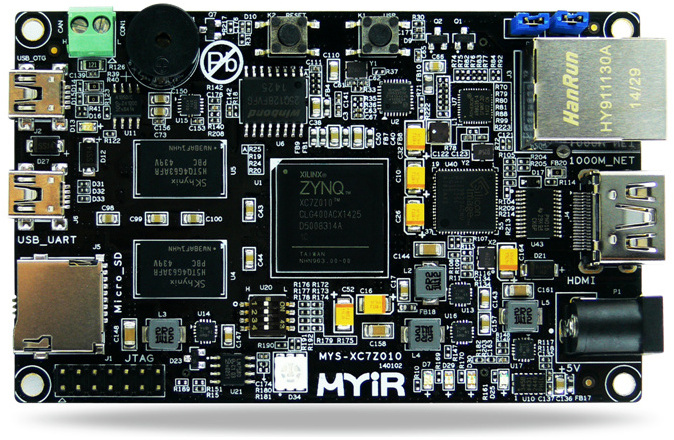
\includegraphics[width=0.5\textwidth]{img/zturn_board.jpg}
  \caption{Płytka Z-turn-Board 7020}
  \label{zturn_board}
\end{figure}

Biorąc pod uwagę parametry, płytka 
charakteryzuje się wysokim stodunkiem ceny do jakości, podstawowa wersja kosztuje 
99\$. Dla porównania płytka Zybo Z7-20 kosztuje 199\$. Zestawienie cen płytek 
zawierających układ Zynq XC7Z010 oraz XC7Z020 znajduje się w Tabeli \ref{tab:ceny}. 

\subsubsection{Interfejsy komunikacji}

Płytka Z-turn posiada interfejsy UART oraz Ethernet, które zostały wykorzystane do 
komunikacji komputera PC z systemem przy użyciu portu szeregowego  
i protokołu SSH (ang. \emph{Secure Shell}). Istnieje również możliwość podłączenia 
wyświetlacza bezpośrednio do płytki przy użyciu portu HDMI. Dodatkowo producent 
oferuje płytkę rozszerzeniową Z-turn IO-Cape (Rys. \ref{iocape}), która zawiera 
porty do podłączenia kamery przez protokół DVP (ang. \emph{Digital Video Port}) 
oraz wyświetlacza LCD. 

\begin{figure}[h]
  \centering
  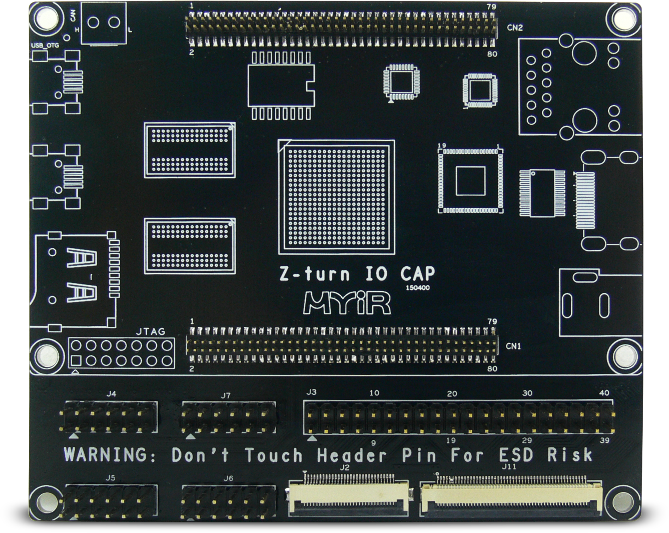
\includegraphics[width=0.5\textwidth]{img/iocape.png}
  \caption{Płytka rozszerzeniowa Z-turn IO Cape}
  \label{iocape}
\end{figure}

\subsection{Kamera}


              % Umożliwia to również łatwą migrację do nowej wersji szablonu:
\newpage % Rozdziały zaczynamy od nowej strony.
\cleardoublepage % Zaczynamy od nieparzystej strony
\pagestyle{headings}

\section{Implementacja}
W początkowej fazie projektu przetestowano wiele różnych modeli ANN w celu znalezienia odpowiedniej architektury sieci do zastosowania w przetwarzaniu obrazów. Początkowo zastosowano splotową sieć neuronową, która przy niewielkiej liczbie parametrów dawała bardzo dobre wyniki klasyfikacji odręcznie pisanych cyfr z bazy MNIST. Jednak w celu zaimplementowania algorytmu w układzie FPGA ograniczono model do postaci architektury MLP. Początkowym założeniem była możliwość zmiany parametrów sieci z poziomu aplikacji.

\subsection{Budowa systemu}

Na początku pracy przyjęto założenie wykonywania uczenia sieci na komputerze PC z wykorzystaniem pakietu \emph{keras}, a następnie eksport modelu w postaci plików tekstowych zawierających parametry sieci. Zbiór obrazów przedstawiających odręcznie pisane cyfry, został podzielono na testowy (10000 obrazów) oraz uczący (60000 obrazów). Ponadto system powinien umożliwiać rozpoznawanie i klasyfikację cyfr na obrazie z kamery w czasie rzeczywistym.

\subsubsection{Schemat blokowy systemu}

System można podzielić na dwie główne części (Rys. \ref{schemat_blokowy}):
\begin{itemize}
  \item aplikacja wykorzystująca pakiet keras, uruchamiana na komputerze PC
  \item część uruchamiana na płytce Z-Turn Board
\end{itemize}

\begin{figure}[!h]
  \centering
  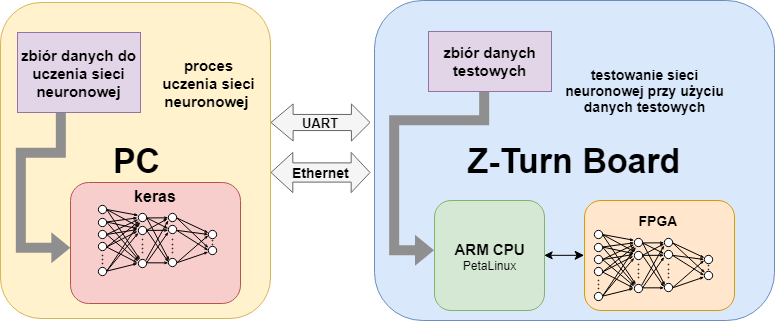
\includegraphics[width=\textwidth]{img/schemat_blokowy.png}
  \caption{Schemat blokowy systemu}
  \label{schemat_blokowy}
\end{figure}

\subsection{Wybór narzędzi}

Użycie w pracy płytki z układem Zynq determinuje użycie narzędzi wspieranych 
przez firmę Xilinx. Zdecydowano się na użycie najnowszej (w momencie rozpoczęcia 
projektu) wersji oprogramowania 2019.2. Producent zaleca\cite{VivadoGuide} instalację 
programu Vivado na jednym ze wspieranych systemów operacyjnych:

\begin{itemize}
  \item Microsoft Windows 7 SP1 Professional (64-bit), English/Japanese 
  \item Microsoft Windows 10.0 1809 Update; 10.0 1903 Update (64-bit), English/Japanese
  \item Red Hat Enterprise Workstation/Server 7.4, 7.5, and 7.6 (64-bit)
  \item SUSE Linux Enterprise 12.4 (64-bit)
  \item CentOS 7.4, 7.5, and 7.6 (64-bit)
  \item Ubuntu Linux 16.04.5 LTS; 16.04.6 LTS; 18.04.1 LTS; 18.04.02 LTS (64-bit)
  \item Amazon Linux 2 LTS (64-bit).
\end{itemize}

\bigskip
W projekcie wykorzystywane było również narzędzie Petalinux, które wymaga 
zainstalowania na maszynie z systemem operacyjnym Linux. Zgodnie z 
dokumentacją\cite{PetalinuxGuide} jest to jedna z trzech dystrybucji:

\begin{itemize}
\item Red Hat Enterprise Workstation/Server 7.4, 7.5, 7.6 (64-bit)
\item CentOS Workstation/Server 7.4, 7.5, 7.6 (64-bit)
\item Ubuntu Linux Workstation/Server 16.04.5, 16.04.6, 18.04.1,18.04.02 (64-bit)
\end{itemize}

\bigskip
Aby zapewnić poprawne działanie narzędzi oraz z racji na sporą popularność i duże 
wsparcie społeczności wybrano dystrybucję Ubuntu 18.04.02 LTS. Przy instalacji 
Petalinuxa warto również zwrócić uwagę, że zalecane jest aż 100 GB wolnego miejsca 
na dysku twardym. 

\subsection{Projekt systemu w środowisku Vivado}

Zdecydowano się na zastosowanie bloków pamięci BRAM do komunikacji pomiędzy 
blokiem IP implementowanym z użyciem HLS a procesorem. Zrzut ekranu przedstawiający 
schemat systemu w środowisku Vivado umieszczono na Rys. \ref{vivado-block-design}.
Znajduje się na nim m.in. blok IP \emph{ZYNQ7 Processing System}, przedstawiający 
procesor, oraz blok \emph{AXI Interconnect}, umożliwiający podłączenie peryferiów 
do procesora. Po podwójnym kliknięciu na blok procesora pojawia się okno, w którym
można ustawić odpowiednią konfigurację układu. 

\begin{figure}[!h]
  \centering
  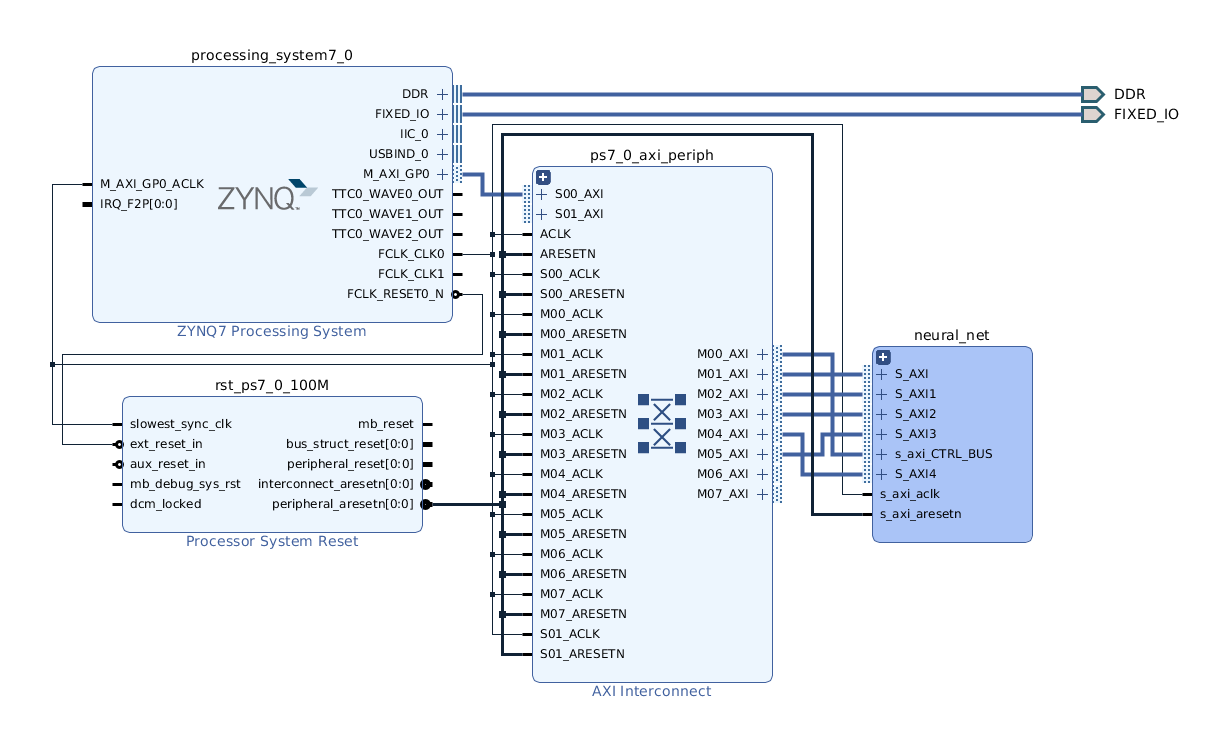
\includegraphics[width=\textwidth]{img/vivado-block-design.png}
  \caption{Schemat systemu przedstawiony w narzędziu Vivado}
  \label{vivado-block-design}
\end{figure}

\subsubsection{Pamięć Block RAM}
Układy FPGA zawierają bloki dwuportowej pamięci BRAM, które można wykorzystać do komunikacji PS -- PL pomiędzy logiką programowalną (ang. PL -- \emph{Programmable Logic}) a procesorem (ang. PL -- \emph{Processing System}).
Zaletą pamięci BRAM jest możliwość równoległego dostępu do danych z dwóch niezależnych portów, jednak ilość pamięci, jaką można wykorzystać, jest mocno ograniczona. W przypadku układu Zynq-7020 znajdującego się na płytce Z-turn jest to 140 bloków po 36Kb (łącznie 4.9Mb). Pamięć BRAM umożliwia dostęp z poziomu sterownika w systemie PetaLinux do danych
przetworzonych przez blok HLS. Zdecydowano się na zastosowanie bloków pamięci BRAM do przechowywania parametrów modelu sieci oraz wejść i wyników obliczeń.

W programie Vivado pamięć alokowana jest przy użyciu bloku 
\emph{Block Memory Generator} i podłączana do procesora dzięki blokom 
\emph{AXI BRAM Controler}(Rys. \ref{vivado-block-neural}) oraz \emph{AXI Interconnect} 
(Rys. \ref{vivado-block-design}). Po odpowiednim podłączeniu bloków pamięci, w zakładce \emph{Adress Editor} można ustawić rozmiar każdego z dodanych bloków BRAM.

\begin{figure}[!h]
  \centering
  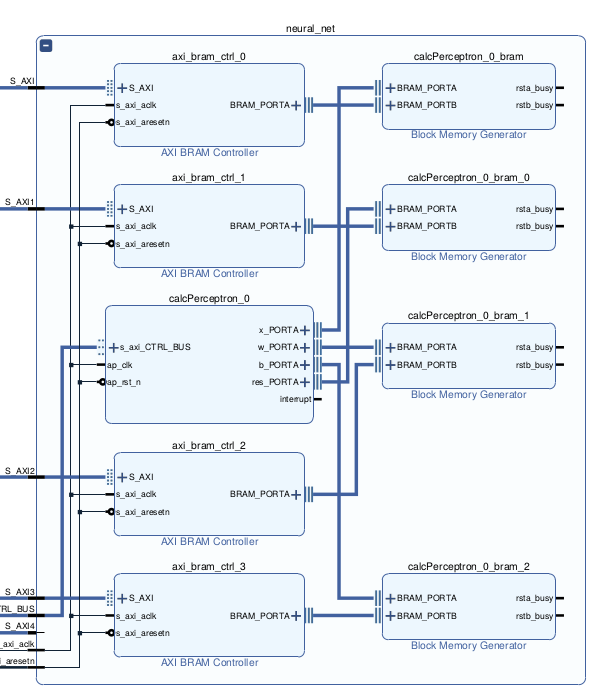
\includegraphics[width=\textwidth]{img/vivado-neuralnet.png}
  \caption{Szczegółowy schemat części systemu \emph{neural\_net}}
  \label{vivado-block-neural}
\end{figure}

\subsection{Wykorzystanie metody HLS}
Przy użyciu metody HLS możliwe jest stworzenie własnego bloku IP (ang. 
Intellectual Property), który następnie jest umieszczany w katalogu IP i można 
go wielokrotnie wykorzystać w projekcie RTL (ang. Register Transfer Level).
Do projektu z użyciem HLS (Rys.\ref{hls_design_flow}) potrzebny jest plik 
z algorytmem w języku C/C++ lub System C, plik testowy napisany w języku C 
(ang. \emph{test bench}) oraz plik z opisem ograniczeń sprzętowych (ang. constraints).
Kolejne etapy projektu z wykorzystaniem metody HLS \cite{hlsXilinxGuide}:

\begin{enumerate}
    \item Kompilacja, wykonanie (symulacja) i debugowanie algorytmu napisanego w języku C
    \item Synteza algorytmu w języku C w implementację RTL
    \item Wygenerowanie raportu i analiza projektu (optymalizacja)
    \item Zweryfikowanie implementacji RTL
    \item Spakowanie implementacji RTL w blok IP
\end{enumerate}


\begin{figure}[!h]
  \centering
  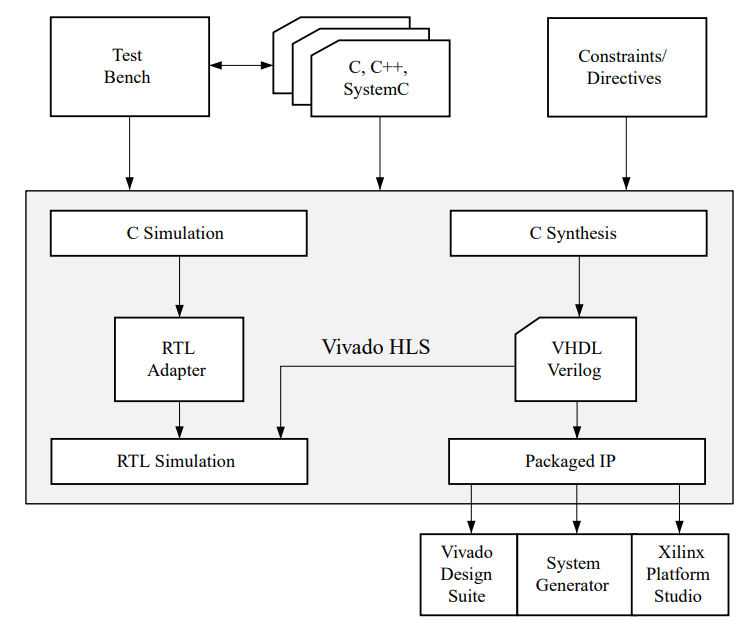
\includegraphics[width=\textwidth]{img/hls_design_flow.png}
  \caption{Proces projektowania przy użyciu metody HLS}
  \label{hls_design_flow}
\end{figure}

Zastosowanie syntezy wysokiego poziomu umożliwia przeniesienie algorytmu napisanego w języku C/C++ lub System C na implementację w układzie FPGA. Dodatkową zaletą metody HLS jest dostępność bibliotek do przetwarzania 
obrazów oraz ułatwiających implementację operacji matematycznych. Podczas pracy nad projektem wykorzystano bibliotekę \emph
{<hls\_math.h>} zawierającą operacje matematyczne (np. funkcję \emph{sigmoid}), podobnie jak biblioteka \emph{<cmath.h>}. 
Obie biblioteki można wykorzystać w implementacji akceleratora HLS, jednak użycie biblioteki \emph{<cmath.h>} może powodować 
powstanie rozbieżnych wyników obliczeń podczas symulacji i syntezy.

Przy tworzeniu nowego projektu w Vivado HLS (Rys. \ref{hls_new_project}) trzeba wybrać 
urządzenie, na którym uruchamiany będzie blok IP. Jeśli płytka nie jest widoczna na 
liście, należy dodać pliki opisujące ją w odpowiednim katalogu, gdzie zostało 
zainstalowane narzędzie Vivado HLS.  

\begin{figure}[!h]
  \centering
  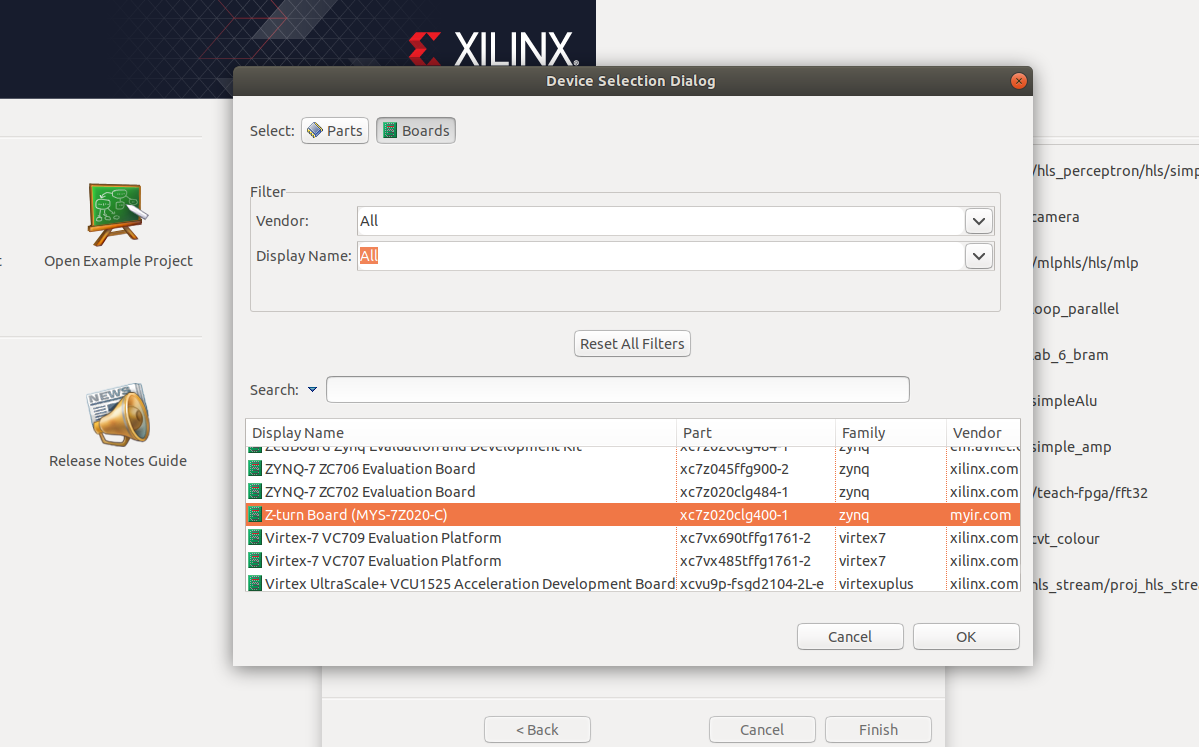
\includegraphics[width=\textwidth]{img/vivado-hls-new.png}
  \caption{Wybór płytki podczas tworzenia projektu w Vivado HLS}
  \label{hls_new_project}
\end{figure}

\subsection{Optymalizacja w Vivado HLS}

Metoda HLS umożliwia optymalizację implementowanego algorytmu pod kątem zużycia zasobów układu FPGA oraz wprowadzanych opóźnień (ang. \emph{latency}). Zaimplementowany algorytm w języku C++ można optymalizować, stosując m.in. następujące dyrektywy:
\begin{itemize}
  \item rozwijanie pętli -- \emph{loop unroll}
  \item przetwarzanie potokowe -- \emph{pipeline}
  \item partycjonowanie tablic -- \emph{array partition}
  \item definiowanie zależności -- \emph{dependence}
\end{itemize} 
Wykorzystanie tych metod umożliwia poprawę wydajności implementacji, jednak zazwyczaj wiąże się ze zużyciem większej ilości zasobów logiki programowalnej. W narzędziu Vivado HLS dyrektywy są implementowane przy użyciu \emph{pragm}, umieszczanych w odpowiednie miejsce w kodzie. Po wprowadzeniu zmian w kodzie i przeprowadzeniu syntezy narzędzie Vivado HLS generuje raport, który umożliwia wstępne sprawdzenie efektów optymalizacji. Na Rys. \ref{hls-report} przedstawiono raport po przeprowadzeniu syntezy implementacji, w której wszystkie pętle są zależne od parametrów modelu ustawionych z poziomu aplikacji. Stąd, widoczne w raporcie znaki zapytania w tabeli \emph{Latency}, gdyż opóźnienia zależą od parametrów funkcji akceleratora. Poza opóźnieniami warto przeanalizować ilość zużytych zasobów, a w szczególności pole \emph{Utilization}, informujące o procentowym zużyciu zasobów. 

W prezentowanym przypadku analiza na poziomie implementacji HLS nie była możliwa ze względu na zbyt dużą ilość zmiennych parametrów, ustalanych na etapie uruchomienia aplikacji. Przeprowadzono testy z poziomu aplikacji w systemie Petalinux dla różnych modeli sieci. Na tym etapie projektu w celu pełnego skorzystania z metod optymalizacji w Vivado HLS, podjęto decyzję o wybraniu modelu sieci, który zostanie na stałe zaimplementowany, bez możliwości zmiany liczby neuronów i warstw sieci.


\begin{figure}[!h]
  \centering
  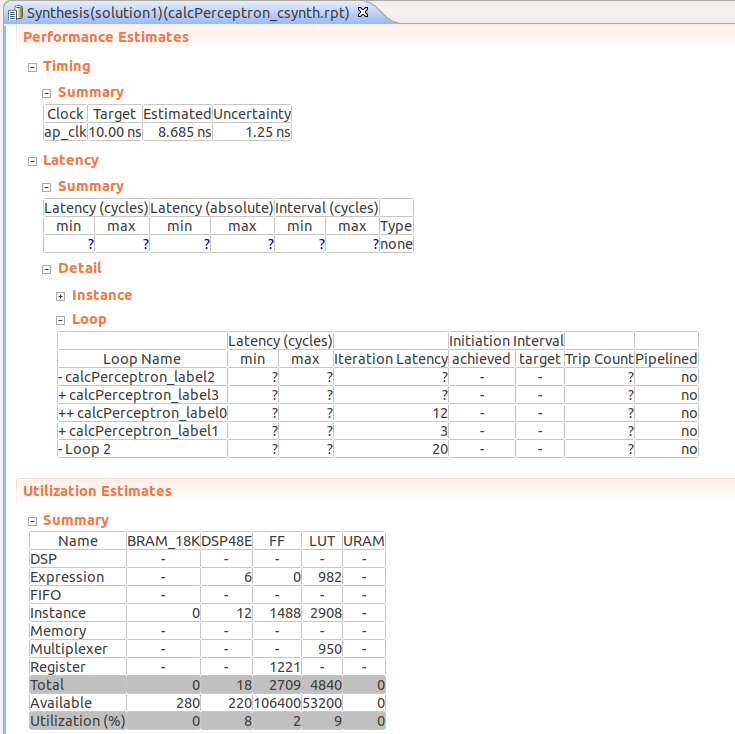
\includegraphics[width=\textwidth]{img/hls-report.png}
  \caption{Raport po przeprowadzeniu syntezy w Vivado HLS}
  \label{hls-report}
\end{figure}


\subsubsection{Rozwijanie pętli}

Każda pętla for w danej implementacji wprowadza pewne opóźnienie (ang. \emph{latency}) w działaniu kodu. W przypadku pętli o 4 iteracjach:
\begin{verbatim}
  multiply:
  for (int i=0; i<3; i++) {
    c[i] = a[i] * b[i];
  }
\end{verbatim}
nie ma możliwości, żeby powyższa pętla wykonała się szybciej niż w 4 cyklach zegara. Aby przyspieszyć wykonanie kodu, można zastosować rozwijanie pętli (ang. \emph{loop unrolling}. W przypadku rozwijania całej pętli wszystkie iteracje danej pętli wykonują się równolegle. W przypadku pętli o wielu iteracjach i ograniczonych zasobach można zastosować rozwijanie częściowe. Użytkownik podaje wartość współczynnika, która informuje o tym, ile iteracji pętli rozpocznie wykonanie jednocześnie.

\subsubsection{Pipeline}
Zastosowanie dyrektywy \emph{Piepeline} umożliwia wykonanie jednej iteracji funkcji lub pętli przed zakończeniem wykonywania poprzedniej. Argumentem dyrektywy PIPELINE jest II (ang. \emph{Initiation Interval}), który informuje o tym, ile taktów zegara będzie pomiędzy rozpoczęciem wykonywania kolejnych instrukcji.
W zależności od złożoności algorytmu i zależności zmiennych w danej pętli, osiągnięcie II=1 może wymagać wprowadzenia zmian w kodzie lub zastosowania dodatkowych dyrektyw.

\subsubsection{Dyrektywa \emph{Dependence}}

Kompilator Vivado HLS automatycznie wykrywa zależności pomiędzy zmniennymi wewnątrz pętli i pomiędzy różnymi iteracjami pętli (ang. \emph{loop-carry dependence}) \cite{hls-pragmas}. W niektórych złożonych implementacjach może dojść do nieprawidłowego zinterpretowania zależności. W tym wypadku można zastosować dyrektywę DEPENDENCE na zmiennej znajdującej się wewnątrz danej pętli lub funkcji, podając jako parametr wartość \emph{false}.

\subsubsection{Partycjonowanie pamięci}

W przypadku posiadania w kodzie zmiennych tablicowych zawierających dużo elementów, można zastosować dyrektywę ARRAY PARTITION, umożliwia podzielenie dużej tablicy na mniejsze lub w całości na pojedyncze elementy. Powoduje to powstanie nowych portów pamięci, których liczba zależy od wartości parametru \emph{factor} podanego w dyrektywie. Partycjonowanie pamięci umożliwia osiągnięcie większego zrównoleglenia dostępu (zapis i odczyt) do pamięci. W przypadku zastosowania dyrektywy:
\begin{verbatim}
  #pragma HLS ARRAY_PARTITION variable=w block factor=4 dim=1
\end{verbatim}
tablica w zostanie podzielona na 4 równe tablice. 

\subsubsection{Arytmetyka zmiennoprzecinkowa}

Kolejną metodą optymalizacji w metodzie HLS jest zamiana arytmetyki zmiennoprzecinkowej (ang. \emph{floating point}) na zapis 
stałoprzecinkowy (ang. \emph{fixed\ point}). Narzędzie Vivado HLS zawiera bibliotekę \emph{ap\_fixed.h}, która ułatwia 
definiowanie zmiennych o wybranym typie stałoprzecinkowym oraz implementowanie operacji matematycznych z użyciem różnych 
typów stałoprzecinkowych. Programista może wybrać liczbę bitów przeznaczonych na część całkowitą i ułamek danej zmiennej, co umożliwia odpowiednie dopasowanie typu zmiennych do wykonywanych obliczeń. Dzięki temu możliwe jest zmniejszenie zużycia zasobów oraz akceleracja obliczeń przy zachowaniu założonej precyzji. Przy dobieraniu liczby bitów w typie stałoprzecinkowym należy wziąć pod uwagę zakres wartości, jakie będzie w stanie przechowywać, co bywa skomplikowane w przypadku złożonych algorytmów z dużą ilością operacji matematycznych. 


\subsection{Zbiór danych wejściowych}

W procesie uczenia oraz testowania poprawności działania modelu sztucznej 
sieci neuronowej wykorzystano zbiór odręcznie pisanych cyfr MNIST 
(ang. THE MNIST DATABASE of handwritten digits)\cite{lecun-mnisthandwrittendigit-2010}. Jest to baza 60000 obrazów do 
przeznaczonych do uczenia sieci oraz 10000 do walidacji. Każdy obraz przedstawia jedną cyfrę w formacie 28x28 pikseli. 
Fragment zbioru MNIST przedstawiono na Rys. \ref{mnist-set}.

\begin{figure}[!h]
  \centering
  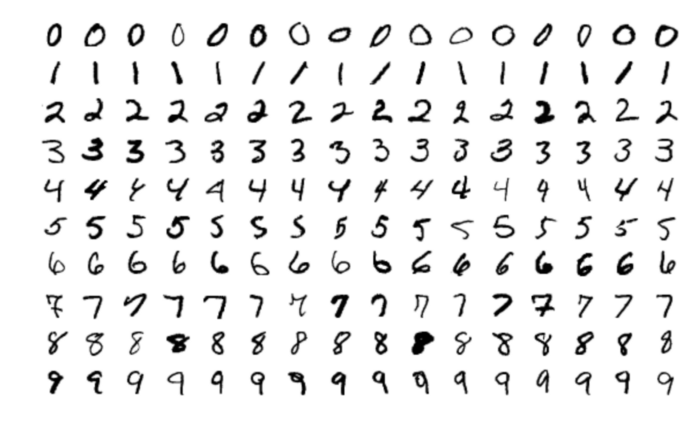
\includegraphics[width=\textwidth]{img/mnist.png}
  \caption{Fragment zbioru odręcznie pisanych cyfr MNIST}
  \label{mnist-set}
\end{figure}

\subsection{Opracowanie modelu ANN}

Przy projektowaniu algorytmu ANN bardzo ważnym aspektem jest odpowiednie dopasowanie modelu do danych wejściowych. 
Najczęściej odbywa się to poprzez wielokrotne testowanie systemu dla różnych parametrów sieci. W tej pracy początkowym 
wyborem była architektura MLP. Dane wejściowe w postaci obrazów 28x28 pikseli są konwertowane na tablicę 784 wartości 
typu \emph{float}. Fragment kodu przedstawia Listing \ref{lst:mlp}. Model zawiera następujące warstwy:
\begin{itemize}
  \item warstwę wejściową (784 wejścia)
  \item warstwę ukrytą (16 neuronów)
  \item warstwę wyjściową (10 neuronów).
\end{itemize}

% Dla dłuższych numerów linii
% potrzebne jest większe wcięcie.
\begin{addmargin}[10mm]{0mm}
  \begin{lstlisting}[
      label=lst:mlp,
      language=python,
      numbers=left,
      firstnumber=55,
      caption={Implementacja modelu ANN MLP z jedną warstwą ukrytą},
      aboveskip=0pt
  ]
model = Sequential()
model.add(Flatten())
model.add(Dense(16, use_bias=True, activation='sigmoid'))
model.add(Dense(num_classes, use_bias=True, activation='sigmoid'))

  \end{lstlisting}
  \end{addmargin}

\subsubsection{Uczenie Sztucznej Sieci Neuronowej}
Podczas uczenia i testowania modelu użyto zbioru MNIST, który zaimportowano, wykorzystując
funkcję z pakietu keras. Dokonano uczenia sieci neuronowej przy użyciu zbioru 60000 
obrazów i testowania modelu, podając na wejście sieci 10000 obrazów. Osiągnięto 
dokładność na poziomie 94,97\%. Na Rys. \ref{keras-accuracy1} przedstawiono, jak zmieniała się dokładność (ang.\emph{accuracy}) w kolejnych epokach dla zbioru uczącego i walidacyjnego.

\begin{figure}[!h]
  \centering
  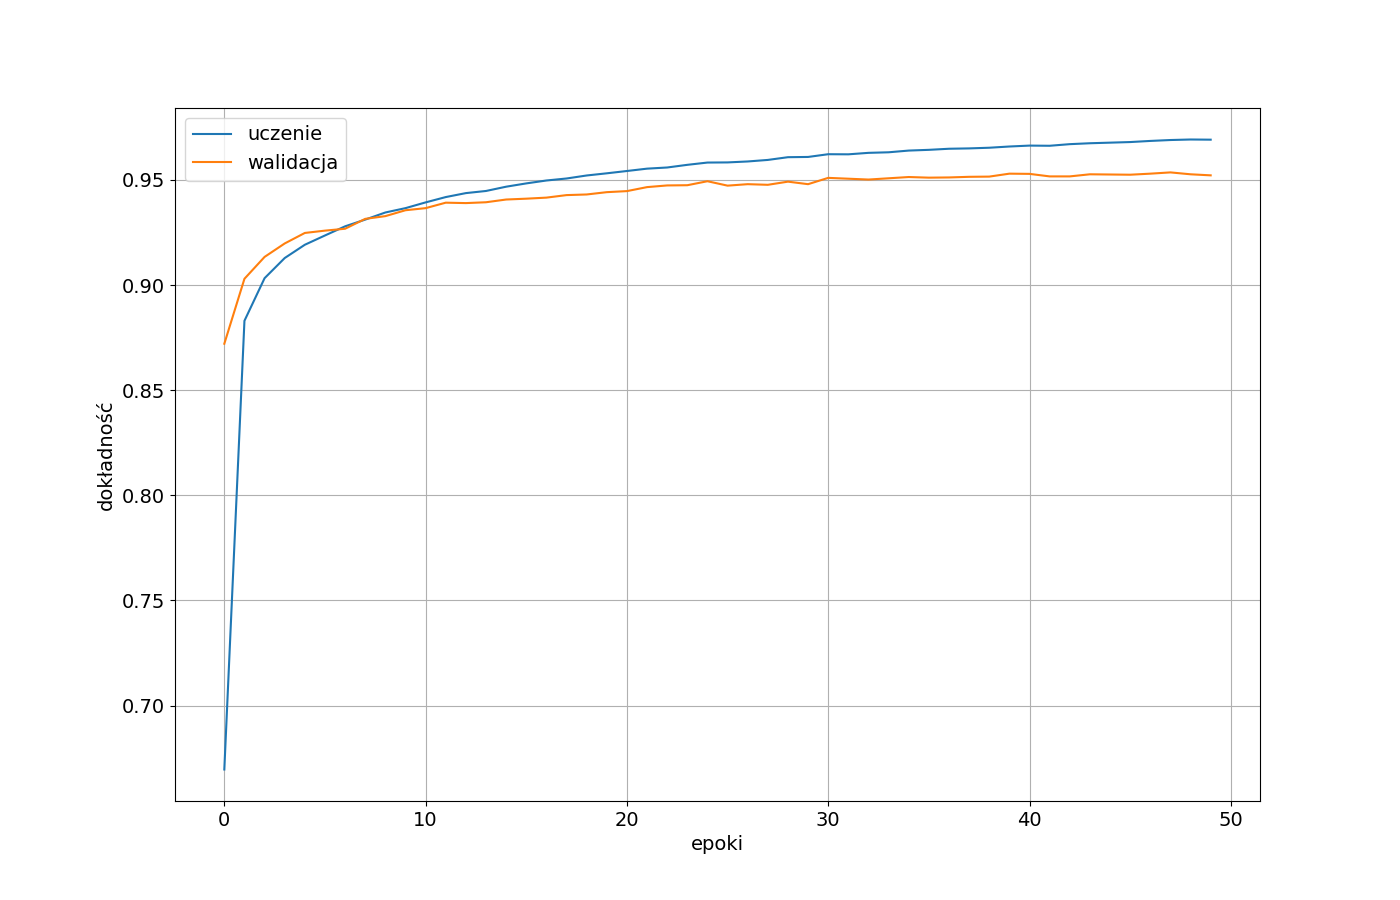
\includegraphics[width=\textwidth]{img/keras-accuracy1.png}
  \caption{Wykres zmian dokładności w kolejnych epokach -- ANN z jedną warstwą ukrytą}
  \label{keras-accuracy1}
\end{figure}

% Wprowadzenie zmian w postaci dodania większej ilości neuronów w warstwie ukrytej nie 
% powodowały zwiększenia dokładności, więc podjęto decyzję o wykorzystaniu tego modelu 
% w dalszej części projektu. 

\subsubsection{Implementacja modelu przy użyciu narzędzia Vivado HLS}

Korzystając z narzędzia Vivado HLS, napisano program w języku C++ implementujący 
zaprojektowany wcześniej model sieci. W procesie uczenia ustalono wartości wag i 
biasów. Dwa główne pliki projektu w narzędziu Vivado HLS to core.cpp, zawierający 
implementację algorytmu ANN oraz test\_core.cpp, który służy do przetestowania
algorytmu po przeprowadzeniu syntezy (ang. \emph{test bench}).   
Pliki zawierające wartości wejściowe, a także wagi i biasy są importowane 
do programu test\_core.cpp. 

Pierwszym etapem jest Symulacja C, która jest wstępną weryfikacją poprawności
algorytmu. Do przeprowadzenia symulacji wykorzystano dane wyeksportowane przy użyciu 
skryptu \emph{keras2fpga.py} i zapisane w plikach hls\_biases.h, hls\_weights.h oraz 
hls\_input.h. Wynikiem symulacji jest plik .log, w którym można znaleźć informacje o
tym, jak przebiegało wywołanie testowanych funkcji.\ref{hls_design_sim}
Symulację w języku C wykonuje się dużo szybciej niż późniejszą symulację RTL, więc
stosuje się ją jako pierwszy etap przed podjęciem dalszych kroków, które zajmują 
więcej czasu.

\begin{figure}[!h]
  \centering
  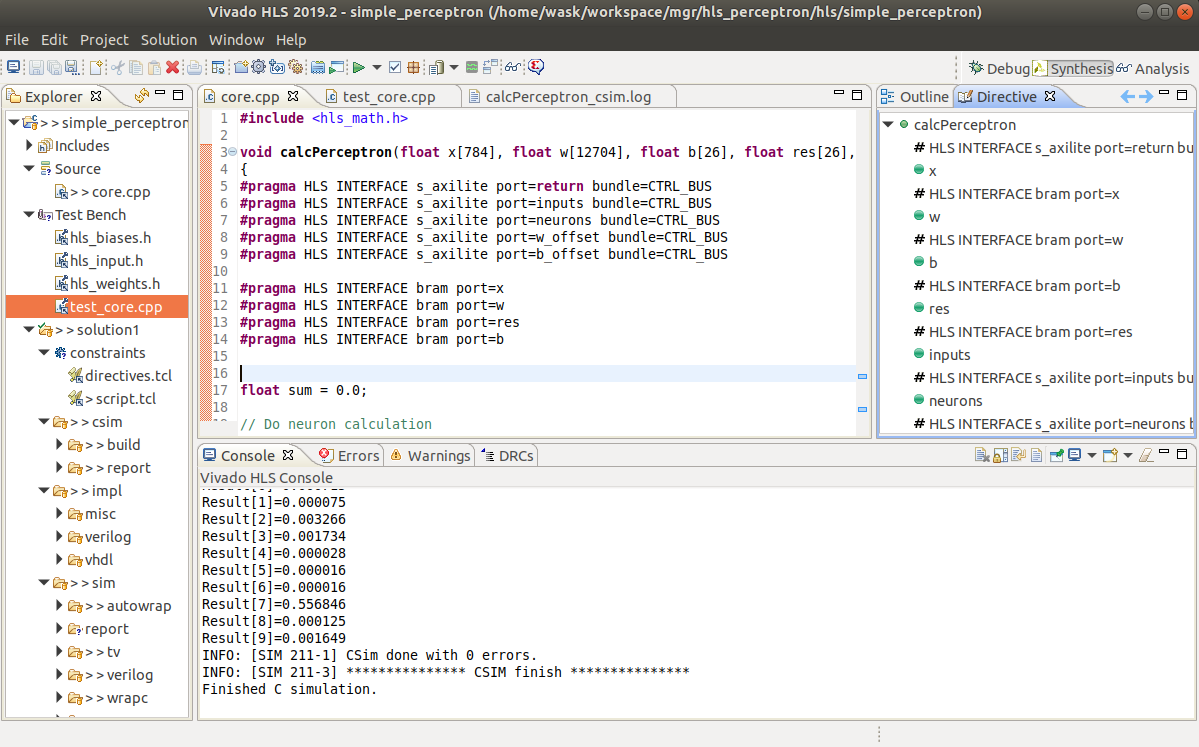
\includegraphics[width=\textwidth]{img/vivado_hls_sim.png}
  \caption{Wynik poprawnie przeprowadzonej symulacji w Vivado HLS}
  \label{hls_design_sim}
\end{figure}


Następnie wykonywana jest synteza oraz kosymulacja, umożliwiająca 
weryfikację poprawności syntezy. Ponadto narzędzie generuje raport, który przedstawia
informacje na temat zużycia zasobów i opóźnień czasowych. Po prawidłowym 
przeprowadzeniu kosymulacji należy użyć opcji \emph{Export RTL}, co umożliwia 
dodanie nowego bloku IP do projektu w narzędziu Vivado.

\subsection{Synteza projektu w narzędziu Vivado}

Aby przetestować działanie nowego bloku IP w narzędziu Vivado HLS, należy dodać i odpowiednio podłączyć blok do 
schematu blokowego (ang. \emph{Block Design}) w narzędziu Vivado. Następnie należy sprawdzić, czy urządzenia zostały 
właściwie zaadresowane w zakładce \emph{Adress Editor} i wprowadzić ewentualne zmiany. Gotowy projekt można poddać 
automatycznej weryfikacji za pomocą funkcji \emph{Validate Design} i uruchomić syntezę i implementację. Po poprawnie 
przeprowadzonej implementacji narzędzie umożliwia otwarcie realizacji sprzętowej projektu (opcja \emph{Open Implemented 
Design}). Zakładka \emph{Timing} (Rys. \ref{impl_design_vivado}) umożliwia sprawdzenie, czy w zaimplementowanym 
projekcie zostały spełnione wymagania czasowe, a w oknie \emph{Device} można zweryfikować jakie zasoby zostały użyte w 
implementacji.

\begin{figure}[!h]
  \centering
  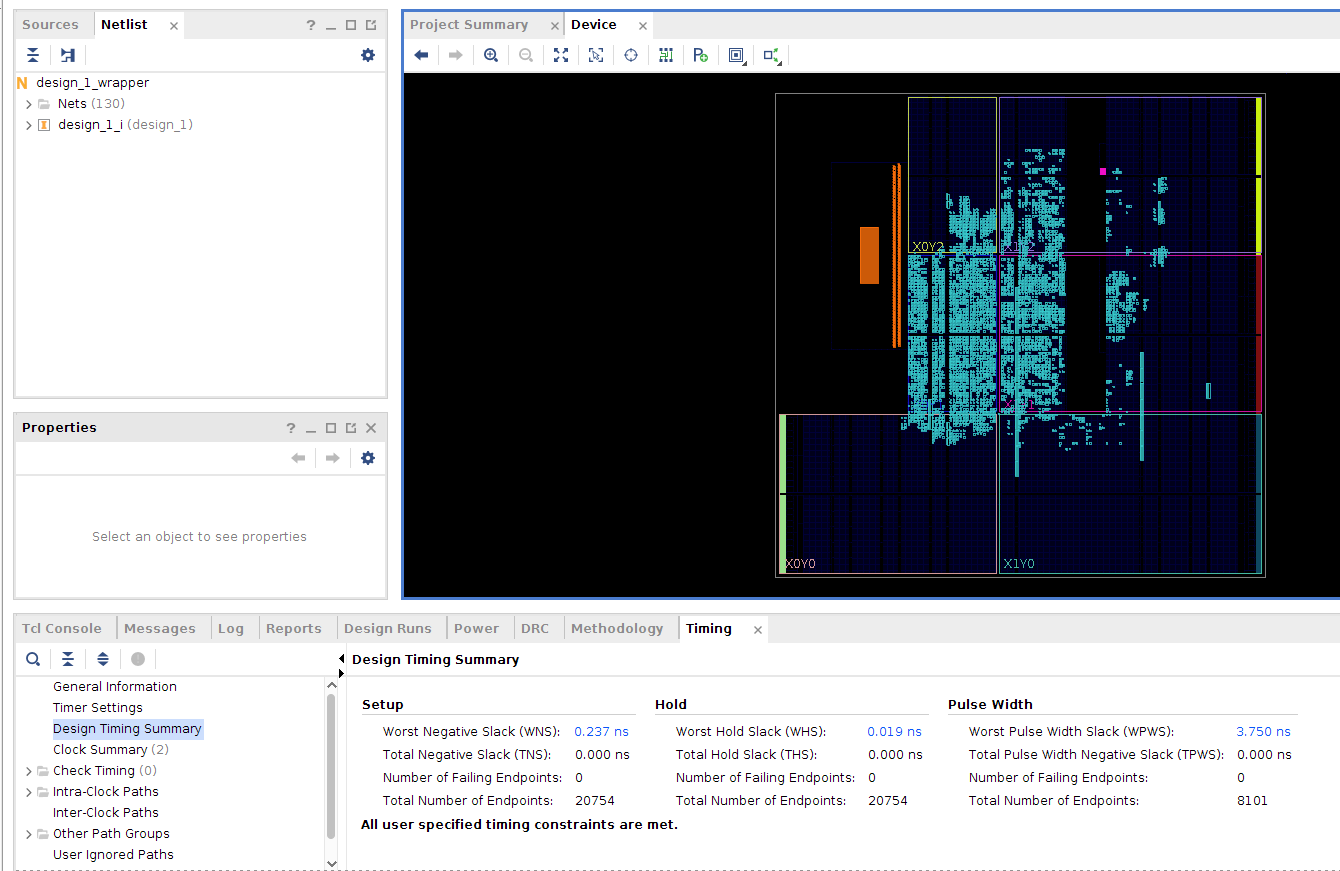
\includegraphics[width=\textwidth]{img/impl-design-vivado.png}
  \caption{Wynik poprawnie przeprowadzonej implementacji w narzędziu Vivado}
  \label{impl_design_vivado}
\end{figure}

Następnym krokiem jest wygenerowanie \emph{Bitstreamu} i eksport sprzętu w postaci pliku z rozszerzeniem \emph{.xsa}.
Dzięki temu projekt sprzętu stworzony w programie Vivado można użyć w narzędziu \emph{Vitis} 
lub \emph{Petalinux}. Aplikacja uruchamiana w trybie \emph{standalone} bez systemu operacyjnego w programie Vitis 
umożliwia szybką weryfikację poprawności działania zaprojektowanego systemu. Dlatego przed przejściem do implementacji 
w systemie Petalinux przystąpiono do stworzenia projektu oprogramowania w programie Vitis.

\subsection{Implementacja przy użyciu narzędzia Vitis}

Po wyeksportowaniu projektu sprzętu w narzędziu Vivado można uruchomić program Vitis. Narzędzie umożliwia stworzenie 
nowego projektu platformy, dzięki opcji \emph{New Platform Project} (Rys. \ref{new-vitis-project1}). Przy tworzeniu 
projektu należy wybrać odpowiedni plik .xsa (Rys. \ref{new-vitis-project2}), wyeksportowany wcześniej z narzędzia 
Vivado. 

\begin{figure}[!h]
  \centering
  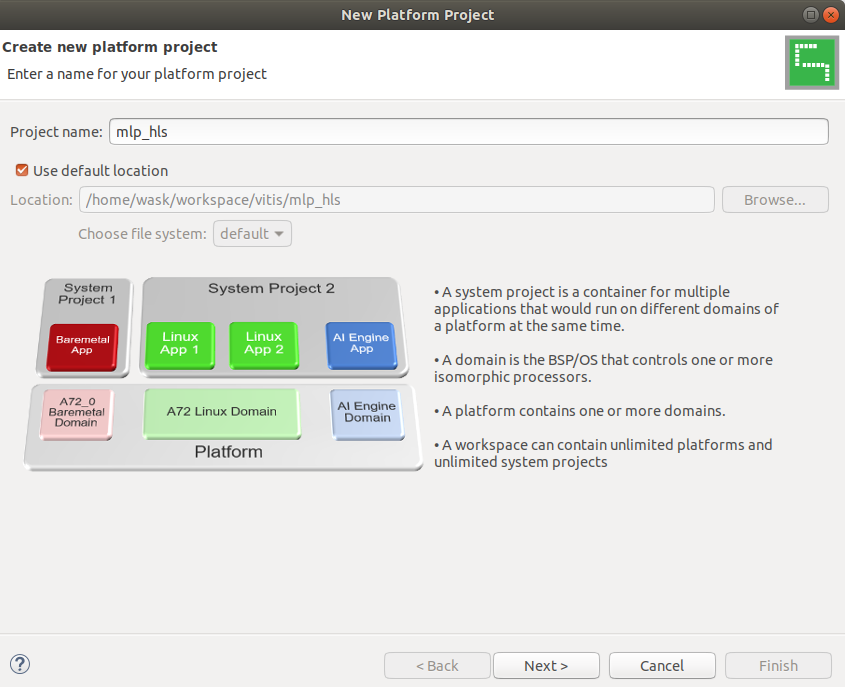
\includegraphics[width=0.9\textwidth]{img/new-vitis-project1.png}
  \caption{Tworzenie nowego projektu w programie Vitis}
  \label{new-vitis-project1}
\end{figure}


\begin{figure}[!h]
  \centering
  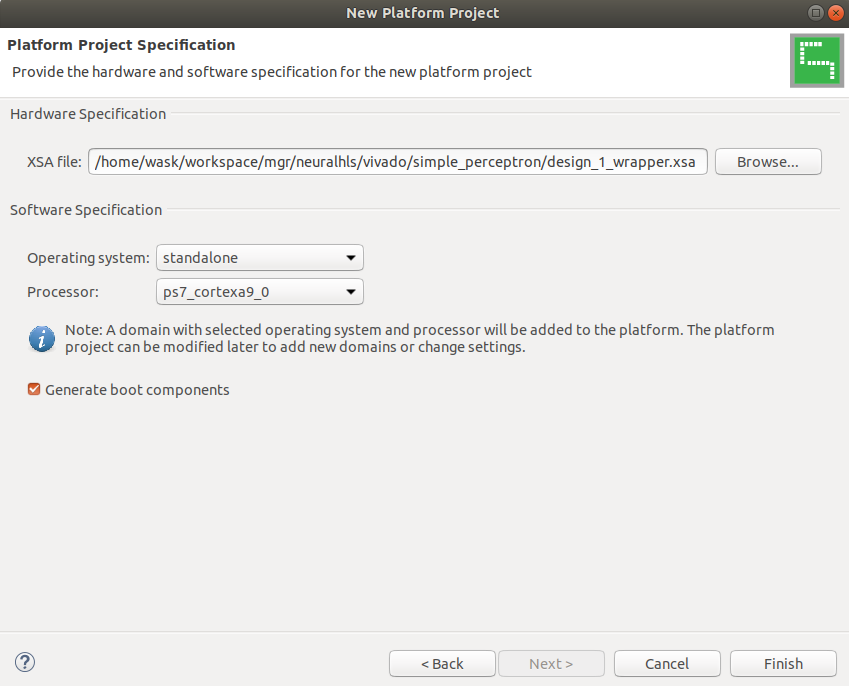
\includegraphics[width=0.9\textwidth]{img/new-vitis-project2.png}
  \caption{Wybór pliku .xsa z opisem konfiguracji sprzętu w programie Vitis}
  \label{new-vitis-project2}
\end{figure}

Następnie należy stworzyć projekt aplikacji, za pomocą opcji \emph{New Application Project} i wybraniu odpowiedniego, 
stworzonego wcześnie projektu platformy. Narzędzie Vitis zawiera szereg aplikacji przykładowych, z których warto 
skorzystać przy uruchamianiu systemu po raz pierwszy. Przed zbudowaniem projektu, aby zapewnić komunikację płytki 
Z-turn Board z komputerem za pomocą konwertera USB-UART znajdującego się na płytce, należy zmienić następujące 
ustawienia BSP (ang. \emph{Board Support Package}) dla domeny \emph{standalone}:

\begin{itemize}
  \item stdin z ps\_7uart\_0 na ps\_7uart\_1
  \item stdout z ps\_7uart\_0 na ps\_7uart\_1
\end{itemize}

Po zbudowaniu projektu platformy można przejść do pisania kodu aplikacji. Warto zaznaczyć, że do uruchomienia i 
debugowania aplikacji na płytce Z-turn Board, potrzebny jest programator JTAG \emph{Xilinx Platform Cable}. Aby 
obejrzeć wyjście standardowe programu, należy otworzyć okno \emph{Vitis Serial Terminal} i wybrać odpowiedni port USB. 
Trzeba również pamiętać o wybraniu odpowiedniej opcji uruchamiania płytki, poprzez ustawienie zworki na JP1 zwarte i 
JP2 rozwarte.

\begin{figure}[!h]
  \centering
  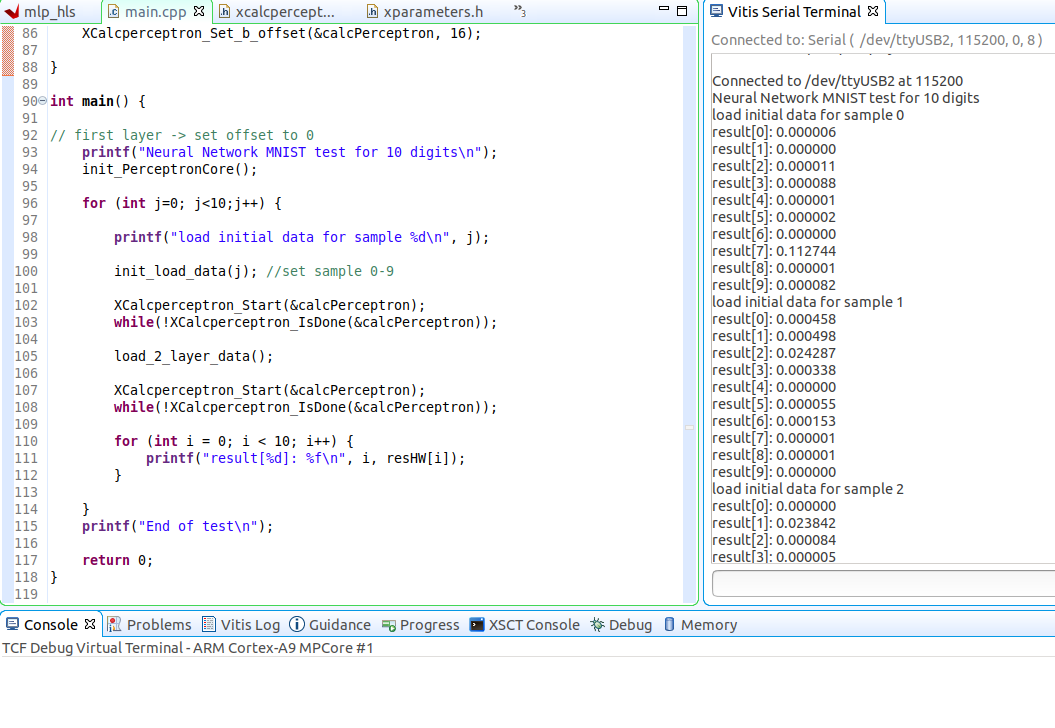
\includegraphics[width=\textwidth]{img/vitis-results.png}
  \caption{Wynik uruchomienia aplikacji w programie Vitis}
  \label{vitis-results}
\end{figure}

Jak widać na Rys. \ref{vitis-results}, algorytm działa poprawnie. Po uruchomieniu i sprawdzeniu poprawności obliczeń w 
programie Vitis można przystąpić do konfigurowania systemu operacyjnego przy użyciu narzędzia Petalinux. 

\subsection{Test z wykorzystaniem systemu operacyjnego Petalinux}

PetaLinux Software Development Kit (SDK) jest narzędziem zawierającym wszystkie niezbędne elementy do budowania,
rozwijania, testowania i wdrażania systemów wbudowanych opartych na systemie Linux. PetaLinux jest przeznaczony głównie 
do systemów, opartych o układy FPGA i składa się z trzech najważniejszych elementów: 

\begin{itemize}
  \item prekonfigurowany obraz binarny systemu 
  \item system Linux konfigurowalny do zastosowania na sprzęcie firmy Xilinx 
  \item PetaLinux SDK zawierający narzędzia służące do projektowania i wdrażania systemu 
\end{itemize}

\subsubsection{Wstępna konfiguracja systemu Petalinux}

Zgodnie z zaleceniami producenta, projekcie wykorzystano wersję narzędzia Petalinux kompatybilną z wersją Vivado -- 
2019.2. Każdorazowo, przed użyciem Petalinuxa należy pamiętać o załadowaniu ustawień przy pomocy komendy:

\begin{verbatim}
  source <katalog-instalacyjny>/petalinux/2019.2/settings.sh
\end{verbatim} 

Narzędzie zużywa dużo przestrzeni dyskowej, jeśli wolnego miejsca będzie zbyt mało, zostanie wyświetlony odpowiedni 
komunikat. Następnie można przejść do tworzenia nowego projektu z ustawieniami domyślnymi dla płytek z układami \emph
{Zynq}:
\begin{verbatim}
  petalinux-create -t project -n <nazwa_projektu> --template_zynq
\end{verbatim}

Projekt sprzętu w programie Vivado został wyeksportowany do pliku z rozszerzeniem \emph{.xsa}. Aby zaimportować plik opisujący konfigurację sprzętu, utworzonego w programie Vivado stosujemy następującą komendę:

\begin{verbatim}  
  petalinux-config --get-hw-description <katalog_projektu_vivado>
\end{verbatim}

Po wywołaniu komendy \emph{petalinux-config} pojawia się interfejs graficzny narzędzia Petalinux, który umożliwia 
zmianę ogólnych ustawień projektu (Rys. \ref{petalinux-config}). Przechodząc do zakładki \emph{Image Packaging 
Configuration} (Rys. \ref{petalinux-config}), można ustawić lokalizację zewnętrznego systemu plików oraz wybrać 
partycję karty sd, na której będzie się znajdował. Stosując opcję -c komendy \emph{petalinux-config} można dostosować 
ustawienia jądra Linuxa (argument \emph{kernel}) oraz systemu plików (argument \emph{rootfs}).

\begin{figure}[!h]
  \centering
  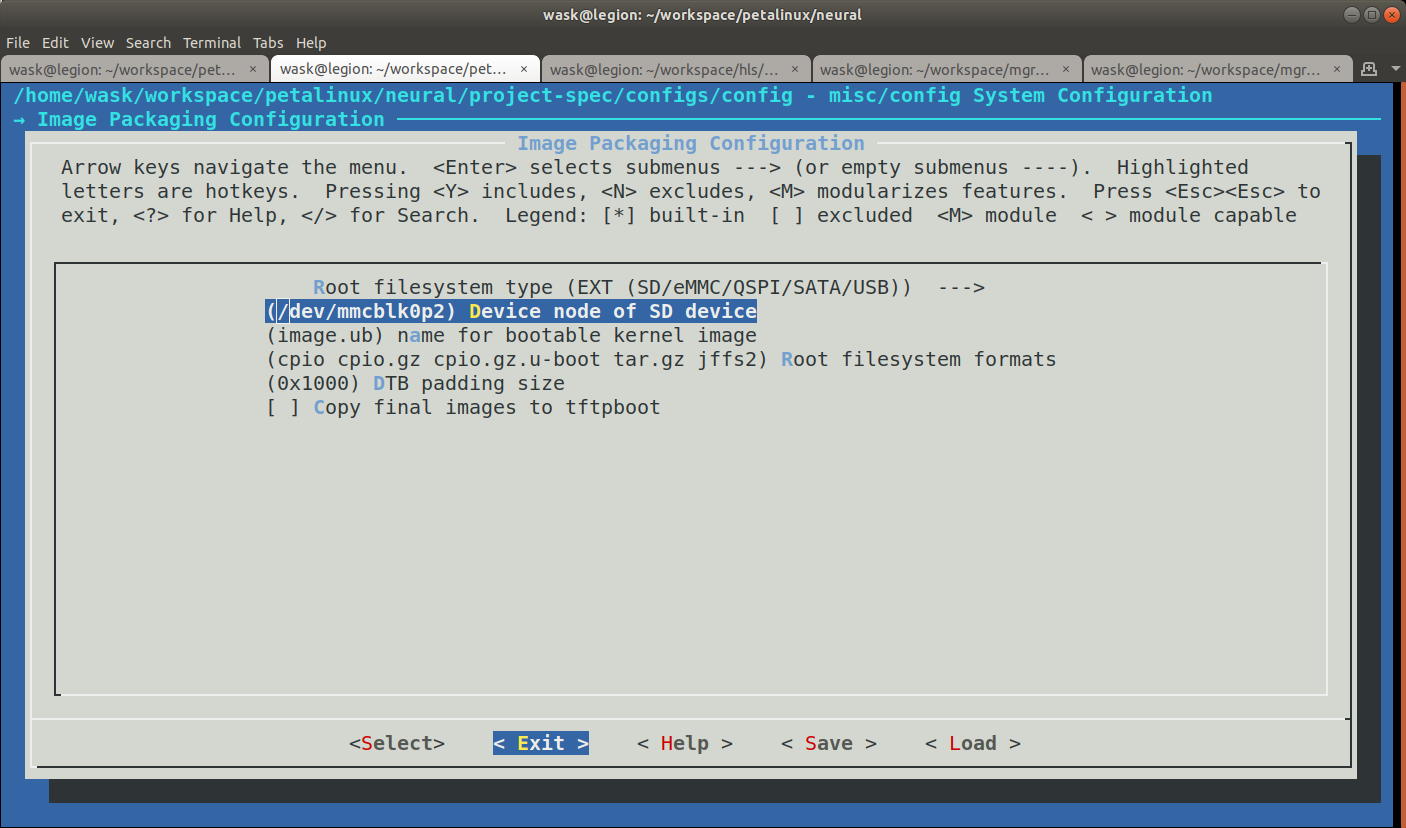
\includegraphics[width=\textwidth]{img/petalinux-config.png}
  \caption{Wstępna konfiguracja przy użyciu funkcji petalinux-config}
  \label{petalinux-config}
\end{figure}

\subsubsection{Konfiguracja jądra systemu Petalinux}

Po wywołaniu komendy \emph{petalinux-config -c kernel} w terminalu pojawia się menu konfiguracyjne jądra systemu 
Petalinux. W oknie jest wiele opcji, jednak najwięcej zmian wprowadzono w zakładce \emph{Device Drivers}. 

W projekcie podjęto decyzję o zastosowaniu kamery podłączonej przy użyciu portu USB. Aby umożliwić aplikacji 
korzystającej z biblioteki OpenCV dostęp do urządzenia, potrzebne były odpowiednie sterowniki \cite{usb-camera} 
dostępne w zakładce \emph{Multimedia Support}. Zastosowany w projekcie moduł kamery MY-CAM002U jest kompatybilny ze 
sterownikiem UVC (ang. \emph{USB Video Class}). W konfiguracji jądra dodano również interfejs V4L2, który daje dostęp 
do modułu kamery z poziomu aplikacji z przestrzeni użytkownika.

\begin{figure}[!h]
  \centering
  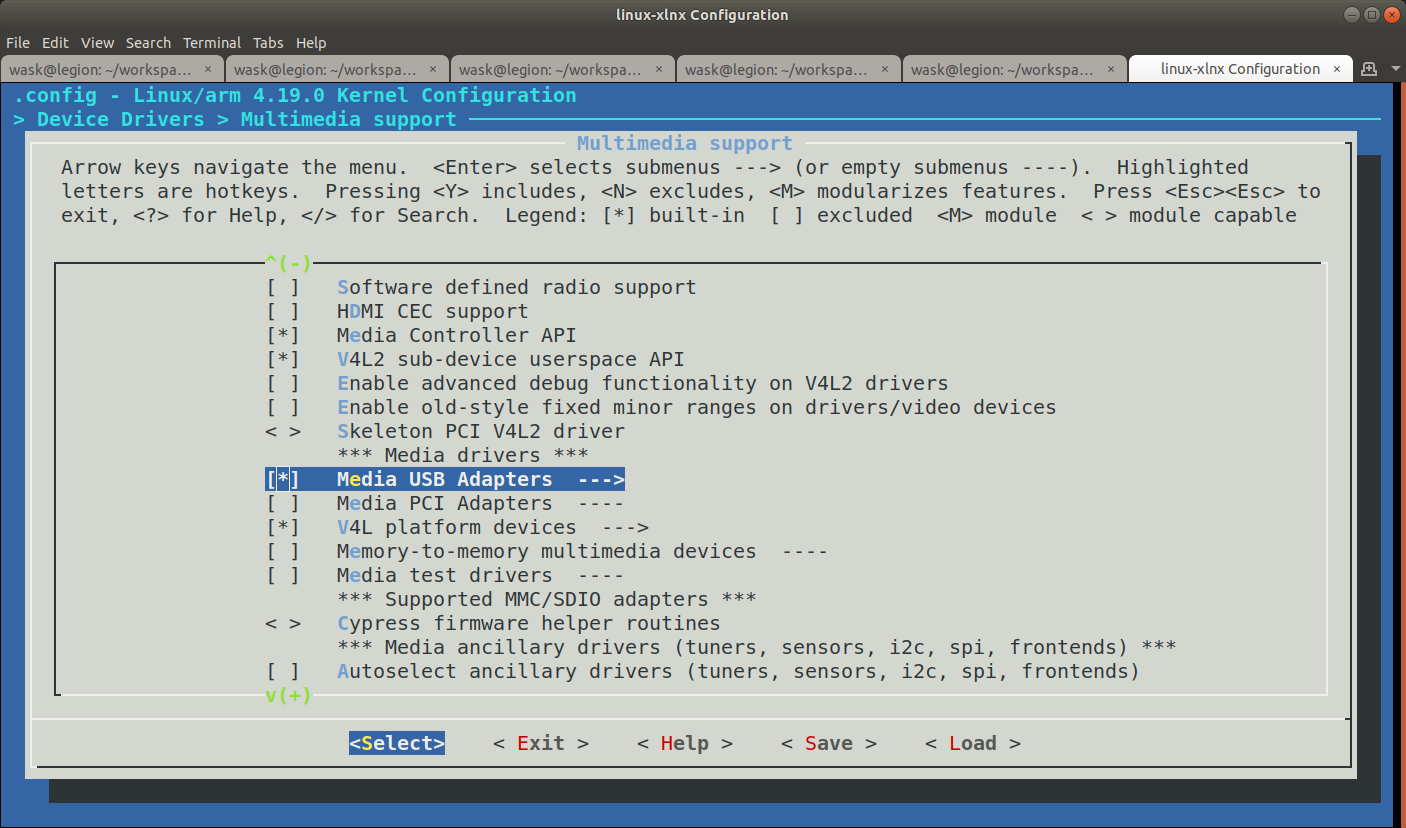
\includegraphics[width=\textwidth]{img/petalinux-config-kernel.png}
  \caption{Konfiguracja jądra PetaLinuxa}
  \label{petalinux-config-kernel}
\end{figure}

Aby uzyskać dostęp z poziomu systemu Petalinux do bloku IP zaimplementowanego w narzędziu Vivado HLS, należy 
zainstalować odpowiednie sterowniki urządzeń lub utworzyć własne. Dla wielu typów urządzeń tworzenie nowego sterownika 
nie jest konieczne. Alternatywnym rozwiązaniem jest zastosowanie sterownika UIO (ang. \emph{Userspace Input Output 
Driver}) \cite{uio-drivers}, który umożliwia dostęp do urządzenia w aplikacji z przestrzeni użytkownika. Znacznie 
upraszcza to proces tworzenia oprogramowania do obsługi urządzenia i zmniejsza ryzyko powstawania trudnych w 
debugowaniu i często niebezpiecznych dla działania systemu operacyjnego błędów. Jednak należy pamiętać, że sterowniki 
UIO nie są przeznaczone dla dowolnego typu sprzętu. Stosuje się je do obsługi urządzeń, generujących przerwania, 
posiadających pamięć, którą można zmapować i sterować urządzeniem poprzez pisanie do tej pamięci. 

\subsubsection{Konfiguracja systemu plików}

Narzędzie Petalinux umożliwia również dostosowanie systemu plików do potrzeb użytkownika. W menu konfiguracyjnym jest 
wiele pakietów i bibliotek do różnych zastosowań. W zakładce \emph{apps} użytkownik ma dostęp do aplikacji, które 
stworzył w obrębie danego projektu. Narzędzie Petalinux umożliwia utworzenie nowej aplikacji przy użyciu komendy:
\begin{verbatim}
  petalinux-create -t apps -n <nazwa_aplikacji>
\end{verbatim}.

W projekcie zdecydowano się na użycie skryptów napisanych w języku Python i biblioteki OpenCV do rejestrowania obrazu i 
wysyłania go poprzez port Ethernet do komputera PC. W tym celu zaznaczono następujące opcje w konfiguracji systemu 
plików:  

\begin{itemize}
  \item python i python-math
  \item python-numpy
  \item packagegroup-petalinux-v4lutils 
  \item packagegroup-petalinux-opencv
\end{itemize}


Kolejnym etapem w procesie konfigurowania systemu Petalinux jest dostosowanie drzewa urządzeń (ang. \emph{device-tree}
. Drzewo urządzeń można edytować za pomocą plików system-user.dtsi oraz pl-custom.dtsi dostępnych w katalogu:

\begin{verbatim}
  <katalog_projektu>/project-spec/meta-user/recipes-bsp/device-tree
\end{verbatim}
W przypadku wykorzystania sterowników UIO należy wpisać w polu \emph{compatible} każdego z węzłów urządzeń (pamięci 
BRAM) wartość \emph{"generic-uio"} \cite{uio-device-tree}. Dostęp do urządzeń jest zapewniony dzięki plikom /dev/uioX, 
gdzie X to numer urządzenia (zaczynając od 0 dla pierwszego urządzenia).

\subsubsection{Przygotowanie obrazu systemu}

Po dostosowaniu pliku \emph{device-tree} można uruchomić kompilację petalinuxa komendą \emph{petalinux-build}.
Gdy system zostanie zbudowany, należy spakować wszystkie potrzebne pliki przy użyciu funkcji \emph{petalinux-package}.
Wynikiem tej operacji są dwa pliki dostępne w katalogu images/linux BOOT.bin i image.ub, które należy przekopiować na
odpowiednią partycję karty sd. Jeśli w konfiguracji Petalinuxa wyłączona została opcja wspierania Initial RAM
filesystem, należy dodatkowo wypakować system plików na drugiej partycji na karcie~sd. Tak przygotowaną kartę sd można
umieścić w slocie na płytce Z-turn, podłączyć zasilanie i uruchomić system.Istnieje opcja kompilacji jedynie wybranej 
aplikacji stworzonej przez użytkownika przy pomocy komendy \emph{petalinux-build -c <nazwa\_aplikacji>}. W przypadku 
wprowadzenia zmian w systemie, przed ponownym wypakowaniem systemu plików, należy sformatować partycję zawierającą 
system plików. 

\subsubsection{Uruchomienie systemu Petalinux}

Komunikacja płytki Z-turn z komputerem PC odbywa się na dwa sposoby:
\begin{itemize}
  \item przez interfejs UART przy użyciu aplikacji Minicom (Rys. \ref{petalinux-boot})
  \item przez port Ethernet za pomocą kilenta SSH 
\end{itemize}
Oba rozwiązania były stosowane równolegle na każdym etapie projektu. 

\begin{figure}[!h]
  \centering
  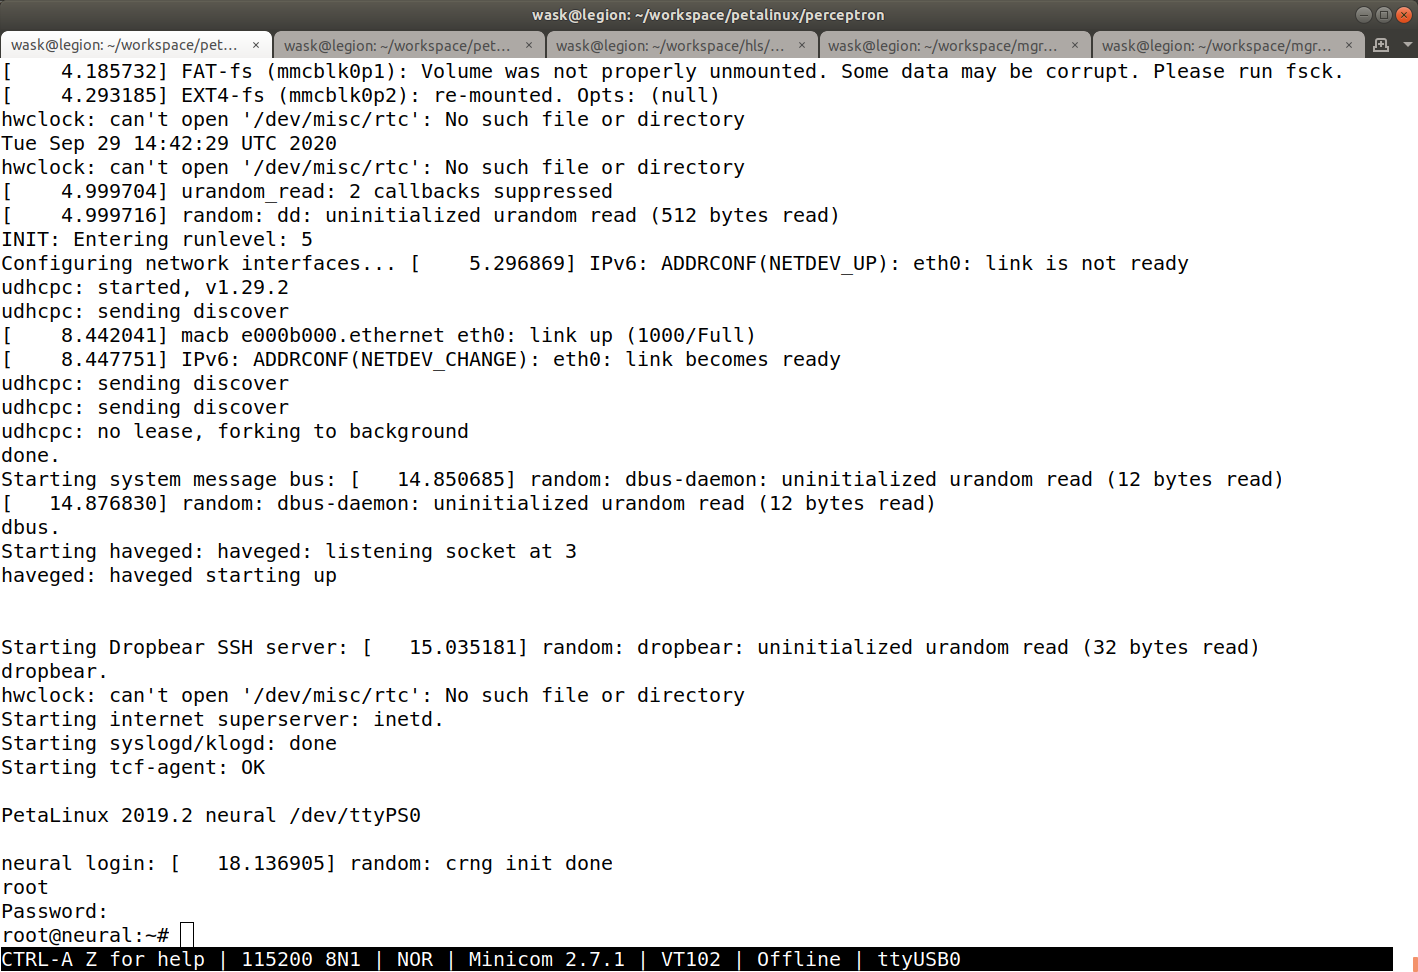
\includegraphics[width=\textwidth]{img/petalinux-boot.png}
  \caption{Uruchomienie systemu PetaLinux}
  \label{petalinux-boot}
\end{figure}

Zaletą konsoli podłączonej za pomocą portu szeregowego jest to, że są w niej wyświetlane komunikaty jądra Linuxa. Ułatwia to debugowanie błędów, które pojawiają się w fazie uruchamiania systemu operacyjnego. Zaletą protokołu SSH jest duża przepustowość i możliwość wysyłania nawet dużych plików.


              % wystarczy podmienić swoje pliki main.tex i eiti-thesis.cls
\newpage % Rozdziały zaczynamy od nowej strony.
\cleardoublepage % Zaczynamy od nieparzystej strony
\pagestyle{headings}

\section{Wyniki i wnioski}

Celem pracy było zaprojektowanie, nauczenie i przetestowanie działania algorytmu Sztucznej Sieci Neurnonowej z użyciem 
układu FPGA oraz porównanie z rozwiązaniem programowym uruchamianym na komputerze PC. Podczas projektu powstało kilka modeli Sztucznej Sieci 
Neuronowej klasyfikującej odręcznie pisane cyfry. Aby porównać rozwiązanie, realizowane w technice HLS z implementacją przy użyciu pakietu \emph{keras}, każdy z modeli poddano testom, które zostały podzielone na dwie części:
\bigskip
\begin{enumerate}
  \item Uruchomienie sieci przy użyciu zbioru testowego 10000 cyfr z bazy MNIST, w celu oszacowania dokładności i 
  szybkości działania algorytmu.
  \item Test wykonany w czasie rzeczywistym przy użyciu modułu kamery.
\end{enumerate}

Wyniki przeprowadzonych testów zostały zestawione w dalszej części rozdziału.

\subsection{Test modelu sieci z jedną warstwą ukrytą}

Wykonano test, podając na wejście sieci 10000 obrazów. Wynik testu, widoczny na Rys. \ref{wynik1} potwierdził poprawność działania algorytmu. Osiągnięto dokładność na poziomie 94,97\%, co pokrywa się z wynikiem uzyskanym z wykorzystaniem biblioteki \emph{keras}.

\begin{figure}[!h]
    \centering
    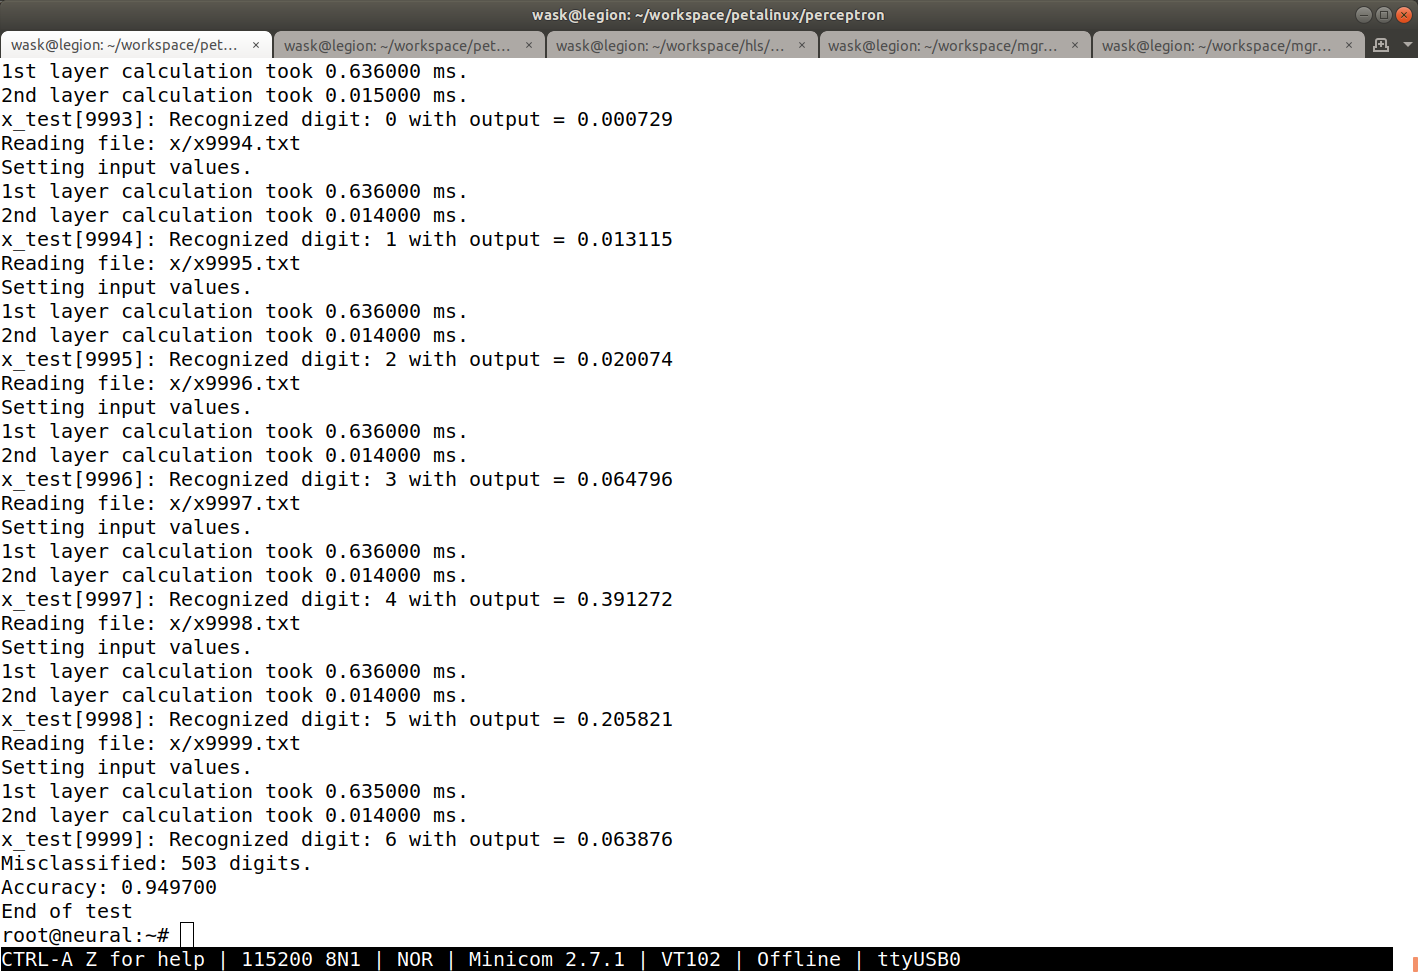
\includegraphics[width=\textwidth]{img/wynik1.png}
    \caption{Wynik testu uruchomionego na SBC Z-turn -- ANN z jedną warstwą ukrytą}
    \label{wynik1}
  \end{figure}


\subsubsection{Test klasyfikacji cyfr z użyciem kamery}

Następnym krokiem był test przeprowadzony w czasie rzeczywistym z użyciem kamery. Rozpoznawanie obiektów na obrazie w czasie rzeczywistym podzielono na 3 części:
\begin{itemize}
    \item detekcja kształtów przypominających cyfry i odrzucenie niewłaściwych obiektów
    \item przygotowanie obrazów do klasyfikacji (odpowiedni rozmiar obrazu i padding)
    \item klasyfikacja obrazów przy użyciu ANN
\end{itemize}

Pierwszą symulację wykonano na komputerze PC przy użyciu biblioteki OpenCV i pakietu \emph{keras}.
Ze względu na sporą ilość obliczeń początkowo zdecydowano się na zarejestrowanie obrazu oraz 
detekcję cyfr przy użyciu biblioteki OpenCV. 

Obraz był rejestrowany w rozdzielczości 640x480 pikseli przy użyciu funkcji \emph{cv2.VideoCapture
(2)}. Następnym krokiem było przekształcenie barwy obrazu na skalę szarości, rozmycie obrazu oraz 
za pomocą funkcji \emph{cv2.adaptiveThreshold} przekształcenie w obraz binarny z odwróconymi 
kolorami. Istotne jest, żeby obraz zawierał białą cyfrę na czarnym tle, ponieważ takie obrazy były 
w zbiorze uczącym.  Następnie użyto funkcji \emph{cv2.findContours}, która zwraca współrzędne 
prostokątów, w które wpisane są kontury znalezione przez algorytm. Po wyeliminowaniu niewłaściwych 
konturów można przejść do przygotowania obrazów do klasyfikacji. 

\begin{figure}[!h]
    \centering
    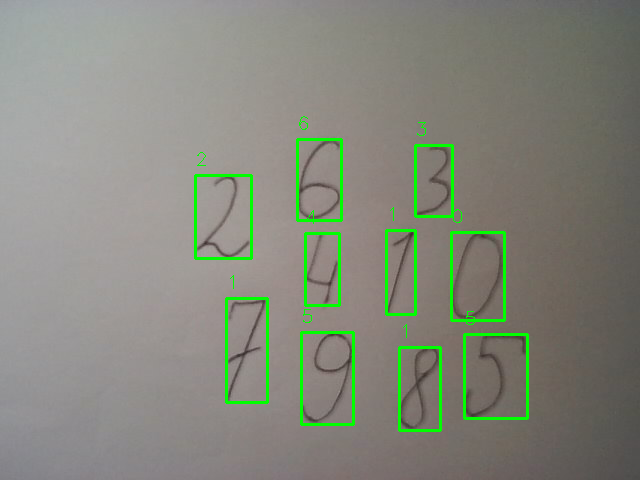
\includegraphics[width=\textwidth]{img/1hid-layer-pc-img.png}
    \caption{Ramka obrazu podczas testu ANN z jedną warstwą ukrytą uruchomionego na PC}
    \label{1hid-layer-pc-img}
  \end{figure}

Odpowiednio przycięty do rozmiaru 28x28 pikseli i wycentrowany obraz ręcznie pisanej cyfry może 
zostać poddany klasyfikacji za pomocą nauczonego wcześniej modelu ANN. W wyniku testu otrzymano 
wyniki przedstawione na Rys. \ref{1hid-layer-pc-img}. 

\begin{figure}[!h]
    \centering
    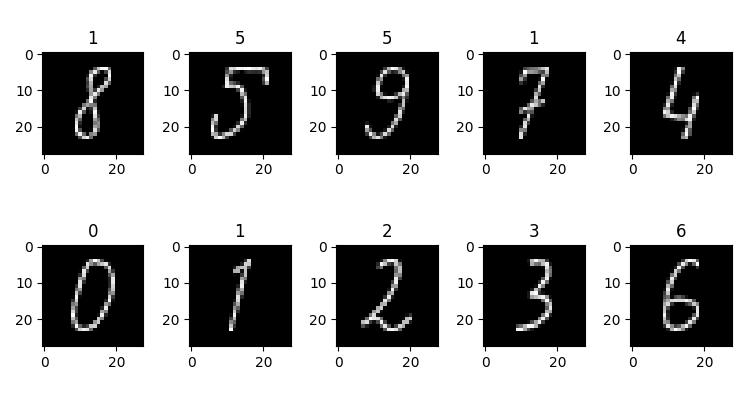
\includegraphics[width=\textwidth]{img/1hid-layer-pc-plot.png}
    \caption{Wynik testu ANN z jedną warstwą ukrytą uruchomionego na PC}
    \label{1hid-layer-pc-plot}
\end{figure}


Rysunek Rys. \ref{1hid-layer-pc-plot} zawiera znalezione na obrazie cyfry i wynik klasyfikacji (nad 
każdą z cyfr). Widać, że 3 z 10 cyfr zostały sklasyfikowane nieprawidłowo, co daje dokładność 
klasyfikacji sieci 70\%.

\subsubsection{Test na płytce Z-turn z użyciem kamery}

W teście na płytce Z-turn zastosowano metodę rejestrowania obrazu taką jak na komputerze PC, jednak 
do rozpoznania cyfr wykorzystano akcelerator obliczeń ANN zaimplementowany w układzie FPGA.  
Aby umożliwić użytkownikowi wyświetlanie obrazu w czasie rzeczywistym, wykorzystano pakiety \emph{pickle} i \emph{socket} do wysyłania kolejnych ramek obrazu przez protokół TCP (ang. \emph{Transmission Control Protocol}). Aplikacja \emph{camera\_server.py} po uruchomieniu na płytce Z-turn oczekuje na połączenie pod zadanym adresem IP 10.42.0.1. Uruchomienie aplikacji \emph{camera\_client} na komputerze PC podłączonym z płytką przy użyciu kabla \emph{Ethernet} powoduje rozpoczęcie rejestrowania obrazu, detekcję i zapisanie obrazów przedstawiających cyfry do plików tekstowych. Działający w tle sterownik UIO \emph{rtdigitrecognition} zawiera mechanizm \emph{inotify}, pozwalający na monitorowanie zmian w pliku \emph{input.txt}, zawierającym dane wejściowe sieci i reagowanie w przypadku zapisania nowych danych. Wynik klasyfikacji odręcznie pisanej cyfry jest zapisywany do pliku \emph{out.txt} i odczytywany w aplikacji rejestrującej obraz, w celu wyświetlenia wyniku przy odpowiedniej cyfrze. Wynik testu przedstawiono na Rys. \ref{1hid-layer-zturn-img}.

\begin{figure}[!h]
    \centering
    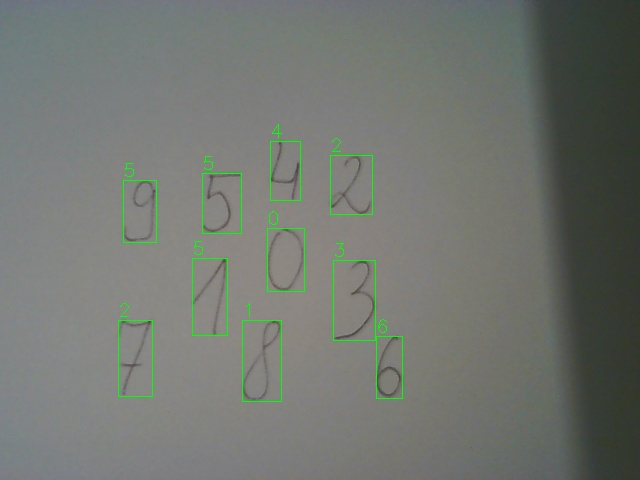
\includegraphics[width=\textwidth]{img/1hid-layer-zturn-img.jpg}
    \caption{Wynik testu ANN z jedną warstwą ukrytą uruchomionego na płytce Z-turn Board}
    \label{1hid-layer-zturn-img}
\end{figure}

Po otrzymaniu wyników pierwszego testu podjęto decyzję o modyfikacji modelu Sztucznej Sieci 
Neuronowej. Pierwszą zmianą było dodanie kolejnej warstwy ukrytej.

\subsection{Test modelu posiadającego dwie warstwy ukryte}

Dodano do istniejącego modelu kolejną warstwę ukrytą zawierającą 64 neurony. Po wykonaniu 50 epok 
otrzymano dokładność na poziomie 97,17\%. Wykres zmiany dokładności w kolejnych epokach 
przedstawiono na Rys. \ref{keras-accuracy2}.

\begin{figure}
    \centering
    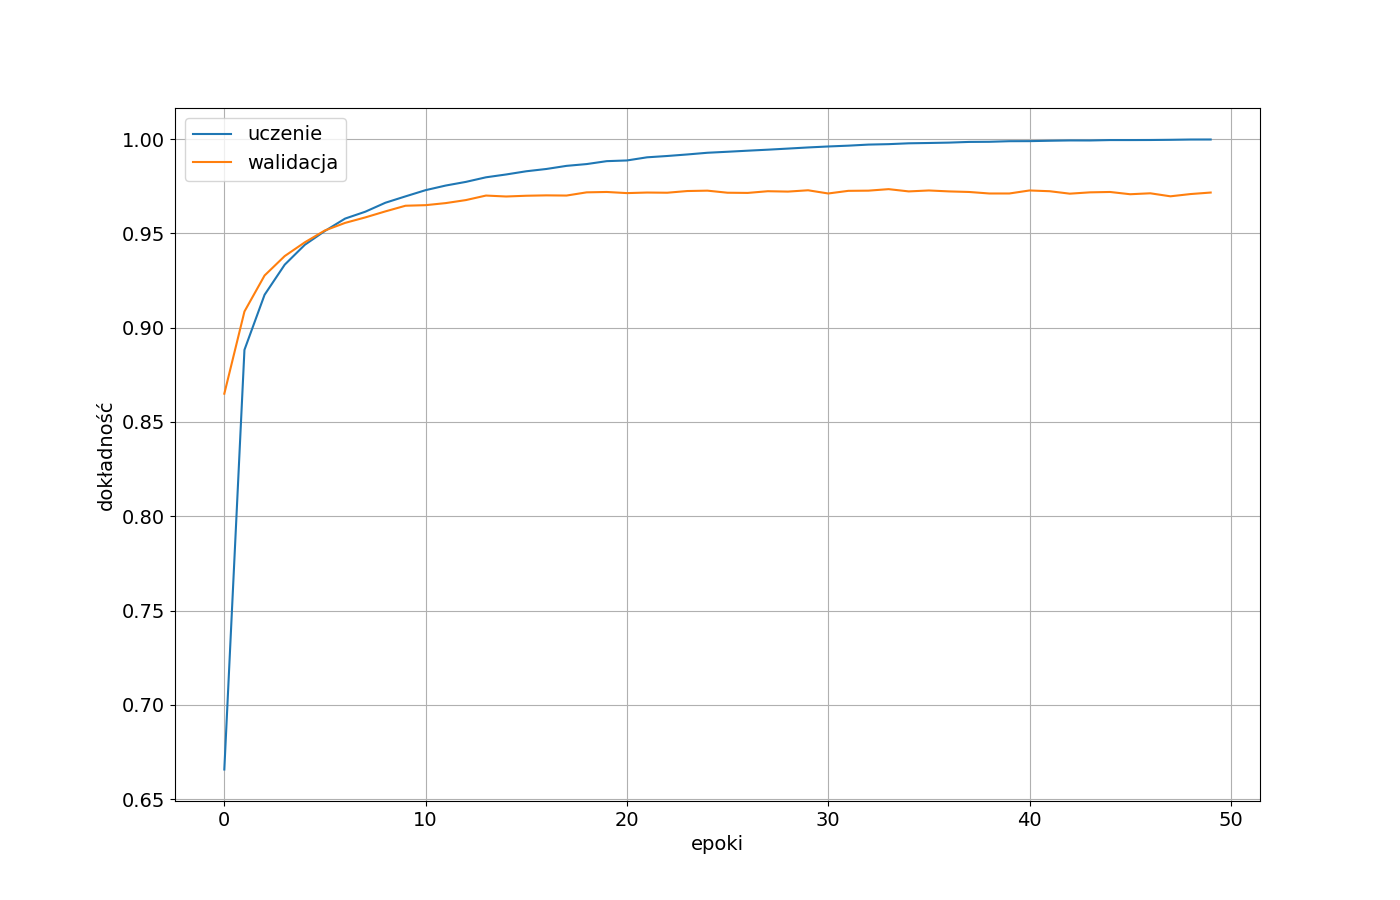
\includegraphics[width=\textwidth]{img/keras-accuracy2.png}
    \caption{Wykres zmian dokładności w kolejnych epokach -- ANN z dwoma warstwami ukrytymi}
    \label{keras-accuracy2}
\end{figure}


\subsection{Implementacja modelu ANN w Vivado HLS}
  Parametry modelu sieci ANN stworzonego, nauczonego i przetestowanego w skrypcie Pythona z użyciem biblioteki keras są przekazywane do funkcji w Vivado HLS. Funkcja \emph{calcPerceptron()} jako argument przyjmuje następujące dane:
  \begin{itemize}
    \item dane wejściowe \emph{x} (obraz odręcznie pisanej cyfry)
    \item wagi sieci neuronowej \emph{w}
    \item biasy sieci neuronowej \emph{b}
    \item adres tablicy na dane wyjściowe sieci \emph{res}
    \item model sieci w postaci tablicy \emph{model} zawierającej:
    \begin{itemize}
      \item liczbę warstw sieci
      \item liczbę wejść sieci
      \item liczbę neuronów w każdej warstwie.
    \end{itemize}
  \end{itemize}

Zmieniając wartości tablicy \emph{model}, użytkownik może zmieniać parametry sieci z poziomu 
aplikacji. Ograniczeniami są rozmiary tablic zawierających parametry sieci, które muszą być 
ustalone na etapie tworzenia projektu oraz ilość pamięci BRAM w układzie \emph{Zynq}.
   
Ponadto z poziomu aplikacji użytkownik ma możliwość ustawienia parametru progu przycinania sieci 
(ang. \emph{pruning threshold}). Dzięki temu możliwe jest wyeliminowanie redundantnych wag sieci, które nie mają znacznego wpływu na wartość wyjścia sieci i skrócenie obliczeń.

\subsection{Dostosowanie parametrów w implementacji HLS}

Implementacja umożliwiająca zmianę parametrów modelu sieci z poziomu aplikacji jest bardzo wygodnym 
rozwiązaniem, umożliwiającym szybkie przeprowadzenie testów dla różnych modeli sieci. Jednak 
zdefiniowanie w implementacji HLS parametrów sieci w postaci zmiennych, spowodowało znaczne 
ograniczenia w możliwościach optymalizacji. 

\subsubsection{Optymalizacja pętli}

W przypadku optymalizacji pętli dwie najczęściej wykorzystywane dyrektywy to PIPELINE i LOOP UNROLL. Gdy pętla jest zagnieżdżona przy użyciu PIPELINE dodatkowo wykonywana jest dyrektywa LOOP FLATTEN, powodująca zamianę pętli zagnieżdżonej w pojedynczą pętlę. Wykonanie dyrektywy LOOP FLATTEN nie jest możliwe na pętli zagnieżdżonej, zawierającej zmienną w warunku zakończenia pętli wewnętrznej.

Pierwszym napotkanym problemem był brak możliwości pełnego rozwinięcia pętli przy użyciu dyrektywy:
\begin{verbatim}
  #pragma HLS UNROLL
\end{verbatim}
spowodowany zapisaniem warunku zakończenia pętli w zmiennej, będącej parametrem funkcji bloku HLS. 

% opisz jakie były ograniczenia 

Aby osiągnąć maksymalną akcelerację obliczeń i optymalizację zasobów zmieniono założenia projektu. Parametry modelu zostały ustalone na etapie implementacji bloku HLS. Dzięki temu możliwe było osiągnięcie znacznie lepszych wyników optymalizacji w narzędziu Vivado HLS.

Następnym problemem związanym z rozwijaniem pętli był komunikat Vivado HLS o braku możliwości wykonania operacji wczytania danych z jednej z tablic spowodowany posiadaniem tylko dwóch portów pamięci BRAM. Sugerowanym rozwiązaniem jest użycie innego bloku pamięci pozwalającego na równoległy odczyt dużej ilości danych lub partycjonowanie tablicy.

\subsection{Arytmetyka stałoprzecinkowa}

Kolejną metodą optymalizacji kodu jest zastosowanie arytmetyki stałoprzecinkowej. Przy użyciu biblioteki \emph{<ap\_fixed.h>} zaimplementowano oddzielne typy dla każdej ze zmiennych reprezentujących parametry sieci. Po wykonaniu analizy raportu dla różnych konfiguracji typów stałoprzecinkowych okazało się, że wprowadzenie arytmetyki stałoprzecinkowej w tym projekcie daje duże zużycie zasobów (ponad 100\%), przy nieznacznym spadku opóźnień. W związku z tym zdecydowano się na wykorzystanie typu zmiennoprzecinkowego.

\subsection{Porównanie czasu wykonania różnych implementacji}

Aby przetestować wydajność klasyfikacji danego modelu sieci w implementacji software'owej wykorzystano metodę \emph{model.predict()}.
Implementacja modelu w HLS z możliwością zmiany parametrów sieci nie dała zadowalających rezultatów. Wyniki dla różnych architektur sieci zestawiono w Tabeli \ref{tab:czas-wykonania}. 

\begin{table}[h] \centering
  \caption{Porównanie czasu wykonania implementacji software'owej przy użyciu pakietu keras z implementacją w układzie FPGA z wykorzystaniem akceleratora HLS -- pierwsze podejście}
  \centering
  \begin{tabular} {c|c|c} \hline \label{tab:czas-wykonania}
      
    implementowany model & aplikacja z użyciem keras & akcelerator HLS\\ \hline
    FC10-sig-FC16-sig-FC16-sig-FC10-sig & 0.572 \emph{ms} & 0.635 \emph{ms} \\
    FC16-sig-FC10-sig & 0.569 \emph{ms} & 0.941 \emph{ms} \\
    FC64-sig-FC16-sig-FC10-sig & 0.535 \emph{ms} & 3.796 \emph{ms} \\
    FC16-sig-FC10-soft & 0.457 \emph{ms} & 0.938 \emph{ms} \\
    FC16-relu-FC10-soft & 0.435 \emph{ms} & 0.942 \emph{ms} \\
    \end{tabular}
  \end{table}

  Wykonanie klasyfikacji przy użyciu pakietu keras daje porównywalne wyniki dla każdego z testowanych modeli. W przypadku użycia sieci zawierającej dużą liczbę neuronów w pierwszej warstwie ukrytej czas wykonania obliczeń znacznie rośnie.


  \subsubsection{Wyniki po wykonaniu optymalizacji HLS}
  Po wstępnych testach zdecydowano zmienić założenia implementacji i dokonać optymalizacji wybranej architektury sieci neuronowej. Wybrano następujący model:

\begin{verbatim}
_________________________________________________________________
Layer (type)                 Output Shape              Param #   
=================================================================
flatten_1 (Flatten)          (None, 784)               0         
_________________________________________________________________
dense_1 (Dense)              (None, 16)                12560     
_________________________________________________________________
dense_2 (Dense)              (None, 10)                170       
=================================================================
Total params: 12,730
Trainable params: 12,730
Non-trainable params: 0
_________________________________________________________________
\end{verbatim}

W wyniku uczenia sieci otrzymano dokładność klasyfikacji na poziomie 94,14\%.

Wybrany model zaimplementowano w programie Vivado HLS. Ustalenie wartości parametrów liczby wejść i neuronów na etapie implementacji HLS dało większe możliwości optymalizacji. Raport z syntezy umieszczono na Rys. \ref{hls-report2}. Widać, że parametr II (ang. \emph{Initiation Interval}) jest duży i jest jeszcze możliwość optymalizacji algorytmu. Zużycie zasobów jest na akceptowalnym poziomie.

\begin{figure}[!h]
  \centering
  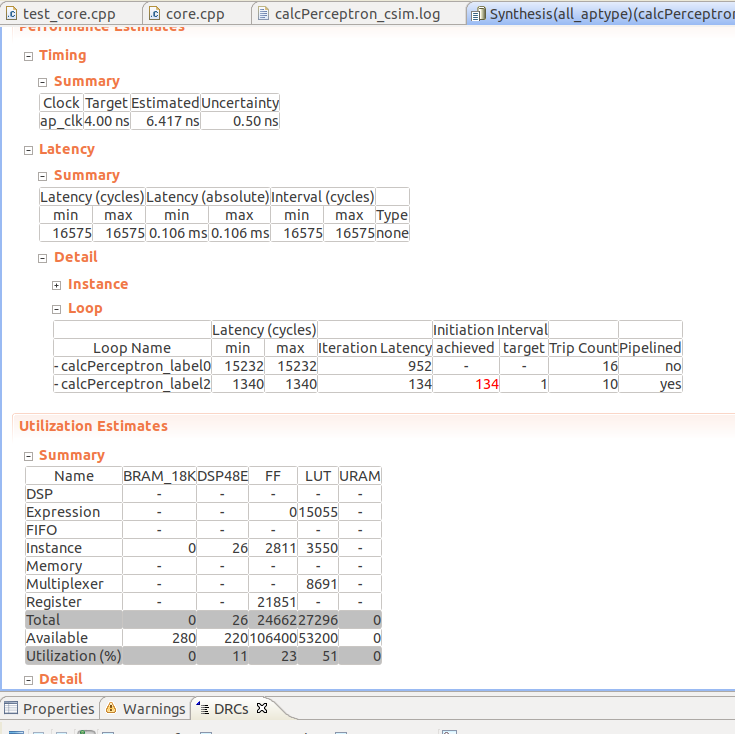
\includegraphics[width=\textwidth]{img/hls-report2.png}
  \caption{Raport po przeprowadzeniu syntezy w Vivado HLS -- drugie podejście}
  \label{hls-report2}
\end{figure}

W wyniku pierwszych testów porównawych otrzymano średni czas klasyfikacji jednego obrazu z użyciem akceleratora HLS 
0.167110 \emph{ms}, a z zastosowaniem pakietu keras 0.463247 \emph{ms}. Daje to akcelerację obliczeń na 
poziomie 2,7.

Po przeanalizowaniu kodu i komunikatów kompilatora Vivado HLS zidentyfikowano problem, powodujący tak duży parametr II. Była to zależność niewłaściwie interpretowana przez kompilator Vivado HLS w pętli wykonującej obliczenia dla danego neuronu.

Aby osiągnąć II = 1 potrzebny był dodatkowy bufor przechowujący sumę iloczynów wejść i wag neuronu w danej iteracji. Dopiero po wyjściu z pętli, gdy sumy iloczynów są policzone dla każdego neuronu w danej warstwie, w kolejnej pętli liczona jest funkcja aktywacji każdego z neuronów. Takie podejście umożliwia osiągnięcie parametru II = 1 dla obu pętli.

Osiągnięto parametr II=1 jednak drastycznie wzrosło zużycie zasobów układu FPGA co widać na Rys. \ref{hls-report3}.

\begin{figure}[!h]
  \centering
  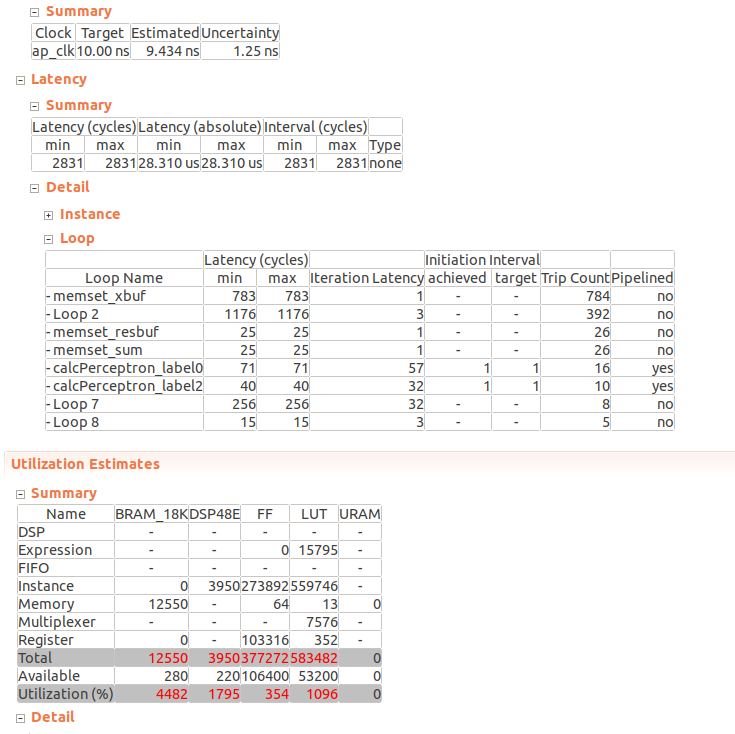
\includegraphics[width=\textwidth]{img/hls-report3.png}
  \caption{Raport po przeprowadzeniu syntezy w Vivado HLS -- minimalizowanie parametru II}
  \label{hls-report3}
\end{figure}

Zajętość elementów BRAM wyniosła ponad 4000\%, co wynika z użycia bramu na przechowanie całej tablicy zawierającej wagi sieci. Aby temu zapobiec, skorzystano z dyrektywy RESOURCE, pozwalającej na wyspecyfikowanie, jakie zasoby będą użyte do zaimplementowania danej zmiennej. Zastosowano dyrektywę zapewniającą implementację tablicy wag jako dwuportową pamięć typu ROM:
\begin{verbatim}
  #pragma HLS RESOURCE variable=w core=ROM_2P_BRAM
\end{verbatim}


\begin{figure}[!h]
  \centering
  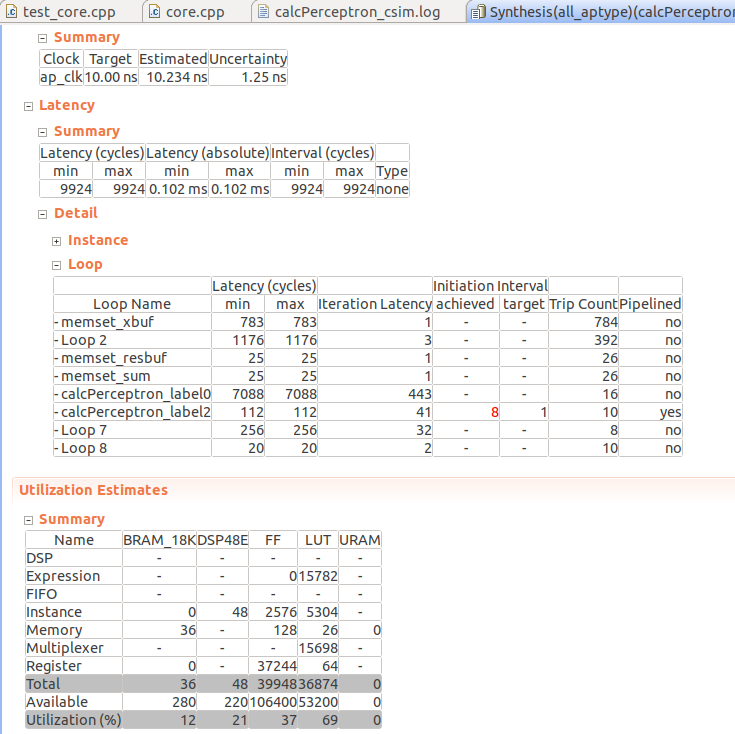
\includegraphics[width=\textwidth]{img/hls-report4.png}
  \caption{Raport po przeprowadzeniu syntezy w Vivado HLS -- minimalizowanie parametru II oraz redukcja zużycia zasobów}
  \label{hls-report4}
\end{figure}

W wyniku syntezy otrzymano rozwiązanie wprowadzające niewielkie opóźnienia i akceptowalne zużycie zasobów. Wyeksportowano blok HLS do narzędzia Vivado i przeprowadzono syntezę i implementację projektu. Po wygenerowaniu Bitstreamu i eksporcie projekt przetestowano rozwiązanie przy użyciu programu Vitis. Ostatecznie osiągnięto wyniki przedstawione w Tabeli \ref{tab:czas-wykonania2}.


\begin{table}[h] \centering
  \caption{Porównanie czasu wykonania implementacji software'owej przy użyciu pakietu keras z implementacją w układzie FPGA z wykorzystaniem akceleratora HLS -- po optymalizacji} W pierwszym wywołaniu otrzymano średni czas wykonania algorytmu 0.145374 \emph{ms}.

  \centering
  \begin{tabular} {c|c|c} \hline \label{tab:czas-wykonania2}
      
      & czas wykonania & dokładność klasyfikacji\\ \hline
     aplikacja z użyciem keras & 0.463247 \emph{ms} & 93,9\% \\
     akcelerator HLS & 0.145374 \emph{ms} & 93,5\% \\
    \end{tabular}
  \end{table}
              % na nowe wersje, a cały tekst pracy pozostaje nienaruszony.
\newpage % Rozdziały zaczynamy od nowej strony.
\cleardoublepage % Zaczynamy od nieparzystej strony
\pagestyle{headings}

\section{Podsumowanie}

Sztuczne Sieci Neuronowe są algorytmem, który bardzo dobrze wpasowuje się w zastosowanie układów FPGA. Akceleracja obliczeń w stosunku do rozwiązań programowych jest możliwa do osiągnięcia. Główne założenia projektu zostały spełnione, stworzono implementację Sztucznej Sieci Neuronowej w układzie FPGA przy użyciu syntezy wysokiego poziomu. Podczas projektu znaleziono elementy implementacji wprowadzające największe opóźnienia i z powodzeniem wyeliminowano lub zmniejszono ich wpływ na czas wykonania algorytmu oraz zużycie zasobów sprzętowych. Osiągnięto rozwiązanie zapewniające akcelerację obliczeń w Sztucznych Sieciach Neuronowych.

\subsection{Wnioski dotyczące techniki HLS}
W dziedzinie rozwijania oprogramowania można zaobserwować tendencję przechodzenia w kierunku rozwiązań wysokopoziomowych.
Ta zależność jest widoczna również w przypadku programowania układów FPGA. Powstają nowe biblioteki i narzędzia usprawniające proces tworzenia implementacji akceleratorów obliczeń. W większości przypadków programista nie musi już posiadać dużej wiedzy o sprzęcie, aby osiągnąć rozwiązanie na akceptowalnym poziomie. Jednak w przypadku złożonych algorytmów bywa, że osiągnięcie implementacji optymalnej, porównywalnej z implementacją w języku HDL jest trudne lub nawet niemożliwe.

\subsection{Możliwości rozwoju projektu}

Użycie w projekcie metody HLS umożliwiło znalezienie elementów implementacji wprowadzających duże opóźnienienia i powodujących duże zużycie zasobów układu FPGA. W końcowym etapie projektu problematyczny okazał się długi czas syntezy i implementacji. 
% czego nie dało się zrobić 

W pracy zaprezentowano zastosowanie Sztucznej Sieci Neuronowej do rozpoznawania obiektów 
znajdujących się na obrazie z kamery podłączanej przez USB w czasie rzeczywistym. Część algorytmu 
odpowiedzialna za detekowanie cyfr na obrazie, była uruchamiana na procesorze ARM przy użyciu 
biblioteki OpenCV co wprowadzało spore opóźnienia i ograniczało wartość FPS oraz maksymalną liczbę 
cyfr możliwych do znalezienia w danym momencie. W przypadku zastosowania systemu do zadań 
klasyfikacji obrazów możliwym usprawnieniem projektu jest zastosowanie kamery podłączanej przez 
interfejs równoległy bezpośrednio do układu FPGA w celu zminimalizowania opóźnień. Dodatkowym 
usprawnieniem może być dalsza optymalizacja algorytmu przy użyciu techniki HLS w celu osiągnięcia maksymalnej akceleracji obliczeń i minimalnego zużycia zasobów logiki programowalnej.

Zaletą rozwiązania zawartego w projekcie jest duża uniwersalność. Dzięki możliwości zmiany 
parametrów sieci w funkcji akceleratora użytkownik ma możliwość dokonywania zmian w modelu ANN z 
poziomu aplikacji. Daje to duże możliwości zastosowania systemu w różnych zadaniach związanych z 
dziedziną \emph{Machine Learning}. Zastosowanie układu FPGA umożliwia znalezienie optymalnego 
rozwiązania zapewniającego kompromis pomiędzy zużyciem mocy, a szybkością działania systemu, co jest bardzo istotne w przypadku zastosowania w systemach wbudowanych.


%--------------------------------------------
% Literatura
%--------------------------------------------
\cleardoublepage % Zaczynamy od nieparzystej strony
\printbibliography

%--------------------------------------------
% Spisy (opcjonalne)
%--------------------------------------------
\newpage
\pagestyle{plain}

% Wykaz symboli i skrótów.
% Pamiętaj, żeby posortować symbole alfabetycznie
% we własnym zakresie. Ponieważ mało kto używa takiego wykazu,
% uznałem, że robienie automatycznie sortowanej listy
% na poziomie LaTeXa to za duży overkill.
% Makro \acronymlist generuje właściwy tytuł sekcji,
% w zależności od języka.
% Makro \acronym dodaje skrót/symbol do listy,
% zapewniając podstawowe formatowanie.
% //AB

\vspace{0.8cm}
\acronymlist
\acronym{ANN}{ang. \emph{Artificial Neural Network}}
\acronym{ASIC}{ang. \emph{Application-Specific Integrated Circuit}}
\acronym{DVP}{ang. \emph{Digital Video Port}}
\acronym{FPGA}{ang. \emph{Field Programmable Gate Array}}
\acronym{GPU}{ang. \emph{Graphics Processing Unit}}
\acronym{HLS}{ang. \emph{High Level Synthesis}}
\acronym{MPSoC}{ang. \emph{Multi-Processor System-on-Chip}}
\acronym{SBC}{ang. \emph{Single Board Computer}}
\acronym{SoC}{ang. \emph{System on Chip}}
\acronym{SSH}{ang. \emph{Secure Shell}}
\acronym{V4L2}{ang. \emph{Video for Linux 2}}



\listoffigurestoc     % Spis rysunków.
\vspace{1cm}          % vertical space
\listoftablestoc      % Spis tabel.
% \vspace{1cm}          % vertical space
% \listofappendicestoc  % Spis załączników

% Używając powyższych spisów jako szablonu,
% możesz tu dodać swój własny wykaz bądź listę,
% np. spis algorytmów.

\end{document} % Dobranoc.
